\documentclass{article}

\usepackage{amsmath}
\usepackage{amsfonts}
\usepackage{amssymb}
\usepackage{multicol}
\usepackage{wrapfig}
\usepackage{mathenv}
\usepackage{multirow}
\usepackage{pdfpages}
\usepackage{vmargin}
\setmarginsrb{2.5cm}{2.5cm}{2.5cm}{2.9cm}{0cm}{0cm}{0cm}{0cm}

\usepackage[utf8]{inputenc}

\usepackage[french]{babel}
\selectlanguage{french}

\usepackage{color}
\usepackage{hyperref}
\hypersetup{pdfborder={0 0 0}, colorlinks=true, urlcolor=blue, linkcolor = darkred}
\usepackage{graphicx}
\graphicspath{{pdf/}} 
\usepackage{listings}
\definecolor{colKeys}{rgb}{0.75,0,0}
\definecolor{colIdentifier}{rgb}{0,0,0}
\definecolor{colComments}{rgb}{0.75,0.75,0}
\definecolor{colString}{rgb}{0,0,0.7}

\usepackage{verbatim}
\usepackage{moreverb}
\usepackage{algorithmic,algorithm}

\lstset{
basicstyle=\ttfamily\small, %
identifierstyle=\color{colIdentifier}, %
keywordstyle=\color{colKeys}, %
stringstyle=\color{colString}, %
commentstyle=\color{colComments}, %
showspaces=false,
}
\lstset{language=java}

% Commandes personnelles %

\definecolor{darkred}{rgb}{0.85,0,0}
\definecolor{darkblue}{rgb}{0,0,0.7}
\definecolor{darkgreen}{rgb}{0,0.6,0}
\definecolor{darko}{rgb}{0.93,0.43,0}
\definecolor{maintitle}{rgb}{0.66,0,0.22}
\definecolor{title}{rgb}{0,0.5,0.5}
\definecolor{quote}{rgb}{0.7,0.7,0.7}
\definecolor{forestgreen}{rgb}{0.14,0.54,0.13}
\definecolor{cyan4}{rgb}{0,0.54,0.54}
\definecolor{firebrick4}{rgb}{0.54,0.1,0.1}
\newcommand{\maintitlecolor}[1]{\textcolor{maintitle}{#1}}
\newcommand{\titre}[1]{\textcolor{title}{#1}}
\newcommand{\tsect}[1]{\titre{\section{#1}}}
\newcommand{\tssect}[1]{\titre{\subsection{#1}}}
\newcommand{\tsssect}[1]{\titre{\subsubsection{#1}}}
\newcommand{\vect}[1]{\overrightarrow{#1}}
\newcommand{\dred}[1]{\textcolor{darkred}{\textbf{#1}}}
\newcommand{\dgre}[1]{\textcolor{darkgreen}{\textbf{#1}}}
\newcommand{\dblu}[1]{\textcolor{darkblue}{\textbf{#1}}}
\newcommand{\dora}[1]{\textcolor{darko}{\textbf{#1}}}
\newcommand{\gre}[1]{\textcolor{darkgreen}{#1}}
\newcommand{\blu}[1]{\textcolor{darkblue}{#1}}
\newcommand{\ora}[1]{\textcolor{darko}{#1}}
\newcommand{\rouge}[1]{\textcolor{darkred}{#1}}
\newcommand{\quotecolor}[1]{\textcolor{quote}{#1}}
\newcommand{\forest}[1]{\textcolor{forestgreen}{#1}}
\newcommand{\cyan}[1]{\textcolor{cyan4}{#1}}
\newcommand{\firebrick}[1]{\textcolor{firebrick4}{#1}}
\newcommand{\ceil}[1]{\left\lceil #1 \right\rceil}
\newcommand{\cdil}[1]{\left\lfloor #1 \right\rfloor}
\newcommand{\term}[1]{\textit{\textcolor{maintitle}{#1}}}
\newcommand{\point}[2]{\item \ora{\underline{#1}} : \textit{#2}}
\newcommand{\bfp}[2]{\item \textbf{#1} : \textit{#2}}
\newcommand{\sumparam}[3]{\sideset{}{_{#1}^{#2}}\sum{#3}}
\newcommand{\sumin}[3]{\sideset{}{_{i=#1}^{#2}}\sum{#3}}
\newcommand{\sumkn}[3]{\sideset{}{_{k=#1}^{#2}}\sum{#3}}
\newcommand{\intin}[3]{\sideset{}{_{#1}^{#2}}\int{#3}}
\newcommand{\stitre}[1]{\noindent\textbf{\underline{#1}} \\}
\newcommand{\R}{\mathbb{R}}
\newcommand{\Z}{\mathbb{Z}}
\newcommand{\N}{\mathbb{N}}
\newcommand{\ualpha}{\vect{u_\alpha}}
\newcommand{\valpha}{\vect{v_\alpha}}
\newcommand{\palpha}{\vect{\Psi_\alpha}}
\newcommand{\npcomp}{\term{$\mathcal{NP}$-complet}}
\newcommand{\npcompl}{\term{$\mathcal{NP}$-complet} }
\newcommand{\cqfd}{\begin{flushright}$\square$\end{flushright}}
\newcommand{\contrad}{\begin{flushright}$\boxtimes$\end{flushright}}
\DeclareMathAlphabet{\mathpzc}{OT1}{pzc}{m}{it}
\newtheorem{de}{D\'efinition}[section]
\newtheorem{note}{Note}[section]
\newtheorem{propriete}{Propri\'et\'e}[section]
\newtheorem{exemple}{Exemple}[section]
\newtheorem{corollaire}{Corollaire}[section]
\newtheorem{interlude}{Interlude}[section]
\newtheorem{rappel}{Rappel}[section]
\newtheorem{rem}{Remarque}[section]
\newtheorem{rems}{Remarques}[section]
\newtheorem{thm}{Th\'eor\`eme}[section]
\newtheorem{lemme}{Lemme}[section]
\newtheorem{illustration}{Illustration}[section]
\newtheorem{pbm}{Problème}[section]
\newtheorem{proof}{Preuve}[section]
\renewcommand{\theproof}{\empty{}} 
\newenvironment{pblm}{\hbox{\raisebox{0.4em}{\vrule depth 1pt height 0.4pt width 5cm}}\begin{pbm}}
{\end{pbm}\hbox{\raisebox{0.4em}{\vrule depth 1pt height 0.4pt width 5cm}}}

%% ALGORITHME

\floatname{algorithm}{Algorithme}
\renewcommand{\algorithmicrequire}{\textbf{Entrée :}}
\renewcommand{\algorithmicensure}{\textbf{Sortie :}}
\renewcommand{\algorithmicif}{\textbf{Si}}
\renewcommand{\algorithmicthen}{\textbf{alors}}
\renewcommand{\algorithmicelse}{\textbf{Sinon}}
\renewcommand{\algorithmicwhile}{\textbf{Tant que}}
\renewcommand{\algorithmicdo}{\textbf{faire}}
\renewcommand{\algorithmicend}{\textbf{fin}}
\renewcommand{\algorithmicreturn}{\textbf{Retourner}}
\renewcommand{\algorithmicfor}{\textbf{Pour}}

%%%%%%%%%%%%%%%%%%%%%%%%%%%%%%%%%%%%%%%%%%%%%%%%%%%%%%%%%%%%%%%%%%%
%%%%%%%%%%%%%%%%%%%%%%%% DEBUT DU DOCUMENT %%%%%%%%%%%%%%%%%%%%%%%%
%%%%%%%%%%%%%%%%%%%%%%%%%%%%%%%%%%%%%%%%%%%%%%%%%%%%%%%%%%%%%%%%%%%

\begin{document}\begin{sffamily}


\includepdf[pages={1},offset=60 -60]{pageGarde.pdf}

\section*{Remerciements}

Je tiens à remercier \textbf{Jef Wijsen}, professeur à l’UMons, qui a accepté d’être mon directeur de stage et qui m’a suivi tout au long de cette période. \\

Je tiens aussi à remercier l'entreprise \textbf{TagExpert} et ses membres pour le parfait accueil qu'ils m'ont offert.
Un remerciement particulier à l'équipe de programmeurs grâce à qui j'ai appris pas mal de choses et dont l'ambiance me manquera.\\

Finalement, je remercie mon maître de stage, \textbf{Aurélien Scoubeau}, sans qui ce stage ne se serait pas aussi bien déroulé
et grâce à qui j'ai compris beaucoup de choses tant au niveau du fonctionnement d'une entreprise qu'à la manière de développer une application
ainsi que sur la plupart des outils avec lesquels j'ai travaillé.


\newpage

\hbox{\raisebox{0.4em}{\vrule depth 1pt height 0.4pt width 10cm}}

\tableofcontents

\vspace*{1cm}

\hbox{\raisebox{0.4em}{\vrule depth 1pt height 0.4pt width 10cm}}

\newpage

%%%%%%%%%%%%%%%%%%%%%%%%%%%%%%%%%%%%%%%%%%%%%%%%%%%%%%%%%%%%%%%%%%%
%%%%%%%%%%%%%%%%%%%%%%%%%%% INTRODUCTION %%%%%%%%%%%%%%%%%%%%%%%%%%
%%%%%%%%%%%%%%%%%%%%%%%%%%%%%%%%%%%%%%%%%%%%%%%%%%%%%%%%%%%%%%%%%%%

\section{Introduction}

Dans le cadre du cours ``Stage en entreprise'' donné en 2\textsuperscript{e} année du Master en sciences informatiques, l'étudiant doit réaliser un stage d'une durée de 10 
semaines minimum dans une entreprise de son choix. Pour ce faire, il doit prendre contact avec l'entreprise et suivre la procédure nécessaire à l'accomplissement du stage. 
Une fois le côté administratif terminé, l'étudiant doit soumettre un cahier des charges à son directeur de stage. Ce cachier reprend toutes les tâches qu'il accomplira au 
sein de l'entreprise et il doit être validé par son maître de stage.  L'étudiant doit également rédiger un rapport de stage à la fin de celui-ci.\\

En ce qui me concerne, j'ai choisi de m'allier avec l'entreprise TagExpert afin d'implémenter une application web de gestion d'affiches électorales pour le compte de la 
FGTB. Ce qui m'intéresse au plus haut point dans ce stage est l'apprentissage des technologies web, telles que le framework MVC Symfony2 ou le javascript, nécessaires à 
l'accomplissement d'une application stable. Aucun cours de développement web n'étant au programme à l'UMons, j'ai décidé de participer à ce stage afin de parfaire mes
connaissances basiques et limitées en la matière et ainsi élargir mes horizons informatiques. \\


Je décris dans le présent document les différentes notions théoriques que j’ai utilisées, les recherches que j'ai effectuées, le travail que j’ai réalisé ainsi que les 
connaissances que cela m'a apporté.

%%%%%%%%%%%%%%%%%%%%%%%%%%%%%%%%%%%%%%%%%%%%%%%%%%%%%%%%%%%%%%%%%%%
%%%%%%%%%%%%%%%%%%%%%%%%%%%% ENTREPRISE %%%%%%%%%%%%%%%%%%%%%%%%%%%
%%%%%%%%%%%%%%%%%%%%%%%%%%%%%%%%%%%%%%%%%%%%%%%%%%%%%%%%%%%%%%%%%%%

\section{TagExpert}

La société \textbf{TagExpert} a été créée en 2007 par les frères \textbf{Blampain} : David et Benjamin. Elle se présente comme une société construisant 
une solution aux besoins de ses clients et concrétisant ces solutions en ligne. Il s'agit donc d'une entreprise totalement orientée web. Elle recueille deux parties majeures 
: 
\begin{itemize}
\item \blu{TagExpert.com} qui est constituée d'une équipe de web-développeurs qui réalisent et mettent en ligne des sites Internet pour les clients,
\item \blu{TagExpert.tv} qui est constituée d'une équipe de réalisateurs/caméramans qui réalisent des vidéos de qualité professionnelle en vue de faire la publicité 
d'entreprises clientes ou d'effectuer des animations flash pour dynamiser un site Internet.
\end{itemize}

De manière concrète, \textbf{TagExpert} met à disposition des services tels que la réalisation de conseil stratégique et \textit{eMarketing}, de sites Internet élégants et 
efficaces, des applications robustes sur mesure, des formations et de la production et post-production vidéos dans le domaine de l'Internet. La société est également une 
fervente supportrice de l'open-source.

\subsection{Qu'est-ce que cette entreprise ?}

\textbf{TagExpert}, c'est avant tout une équipe, une communauté qui défend ses valeurs propres, toutes découlant d'un attachement profond à l'innovation et à l'honnêteté : 
\begin{enumerate}
\item \textbf{L’excellence} : basée sur l’amélioration continue et une recherche poussée d’efficacité et d’efficience, elle donne le goût du défi et permet la poursuite 
d’objectifs ambitieux. Elle garantit également une qualité maximale aux projets des clients.
\item \textbf{L’ouverture d’esprit } : véritable leitmotiv avec l’excellence, il s'agit de donner un regard élargi sur la diversité des opinions, des modes de pensées, mais 
aussi des outils technologiques.
\item \textbf{La flexibilité} :  la structure de la société très souple et leur ouverture leur permettent d’être à l’écoute des projets sans aucun a priori ni solution toute 
faite, ce qui se traduit par la recherche de solutions originales parfaitement adaptées aux désirs des clients.
\item \textbf{La fidélité} :  il n'y a pas d'honneur sans fidélité ni loyauté à l'égard de certains projets et de ceux qui les partagent. La fidélité symbolise la nécessité 
incontournable de tenir ses promesses et remplir ses engagements.
\item \textbf{La confiance} :  corollaire de la fidélité, c’est la base des relations commerciales efficaces et durables. L'attitude de TagExpert envers leurs clients, 
partenaires et employés est caractérisée par la création et l’entretien d’une confiance mutuelle.
\end{enumerate}

Les valeurs de \textbf{TagExpert} sont portées par leur esprit d’équipe et par leurs applications. Leur travail a d’ailleurs été récompensé par l’obtention du Prix Scientifique de la 
Vulgarisation du savoir au travers des technologies de l’information et de la communication par le CEPULB de l’Université Libre de Bruxelles. \\

\subsection{Qui sont-ils ?}

L’équipe de \textbf{TagExpert} est composée de développeurs, designers, monteurs multimédia, architectes Web et consultants. Les formations des équipes sont 
multidisciplinaires. Selon les besoins des clients, celles-ci s’agrandissent avec leurs partenaires également spécialisés.\\
L'équipe se compose de personnes à la tête d’une expérience de 3 à 7 ans dans les métiers du web. Ceux-ci disposent de cursus éducationnels, allant du Bac+3 au Bac+7 dans 
les matières suivantes : communication, économie, développement informatique, infographie, psychologie, image et son numériques, eBusiness, eMarketing, multimédia, 
eCommerce, gestion d’entreprise, philosophie, stratégie et marketing ; et ce, suivis dans diverses institutions. \\

Pouvoir affirmer que l'on peut construire une relation d'affaires, un projet informatique ou une recherche spécifique uniquement par le savoir d'une et d'une même personne, 
voire d’une seule entité commerciale, est révolu ; autrement dit, le savoir universel n'existe plus. C'est pour cette raison que \textbf{TagExpert} s'entoure de spécialistes 
dans d'autres domaines informatiques et des technologies web, le cas échéant. Ainsi les projets des clients peuvent toucher d’autres technologies comme : Flash, 
Actionscript, Vb.Net, Java et eMarketing plus poussé. Le projet sera donc géré par une équipe multidisciplinaire et trans-générationnelle vous assurant un résultat optimal.

\subsection{Historique}

En 2007, les frères Blampain ont mis en commun des compétences distinctes et complémentaires afin de créer la société TagExpert. L'aîné, David Blampain est gestionnaire et 
commercial, le cadet, Benjamin Blampain est développeur informatique et technicien. Dès leur tendre enfance, ils ont manipulé dans tous les sens des PC et des MAC. \\

\textbf{Benjamin Blampain}, passionné d'informatique depuis son \textit{Apple II}, a fait ses premières armes aux productions du Dragon "Dragone SA" après être sorti de 
Namur, diplôme d'informatique de gestion en poche. Responsable du développement des applications Intranet chez Franco Dragone, il est également chargé de missions pour 
mettre en place un cellule de support infrastructure pour les travailleurs américains et canadiens du groupe. Durant ce temps, il se forme également chez 
\textbf{Anaska France} \textit{(un des leaders des formations Open-Source en France)} via les formations PHP Expert.
Il participe ensuite à des conférences internationales sur les outils Open-Source comme CakePHP, Drupal pour renforcer la position Open-Source de la société. \\

Diplômé de la Faculté Warocqué à Mons (2001) et de la Solvay Business School (2003), \textbf{David Blampain}, quant à lui, a commencé sa vie active dans une société 
pharmaceutique très organisée, Quality Assistance s.a.. Il en a tiré un maximum d’enseignements d’un point de vue gestion, commercial et ressources humaines.

Par la suite, TechnocITé, sous couvert de l’Union Européenne pour le programme Prométhée II, a fait appel à ses services en tant que responsable du service e-Business. Cette 
mission consistait à aider et à coacher des sociétés Wallonnes à se développer au niveau informatique et Web. David a ainsi aidé plus de 400 sociétés lors de son mandat de 
manager, gérant une équipe pouvant aller de 3 à 9 personnes, tant en Wallonie qu’en Tunisie. David a aussi été mandaté exceptionnellement comme chercheur à l’ULB – CIERL – 
Faculté de Philosophie et Lettres dans les matières des technologies Web et reste à l’heure actuelle Conseiller Scientifique. Il a reçu le prix scientifique CEPULB pour ses 
recherches se rapportant à la vulgarisation du savoir utilisant les nouvelles technologies.  Il reste conseiller en matière technologiques pour le CIERL de l’ULB et est 
assistant du professeur B. Decharneux à la chaire d’éthique des affaires de l’ULB depuis 2003. (Solvay Business School, Faculté Polytechnique et VUB).

Etant ainsi bien armés et riches d’une jeune mais vaste expérience, les deux frères créent TagExpert sprl en 2007. Autour de ces deux personnalités complémentaires, une 
équipe dynamique de professionnels qualifiés est venue se construire. Celle-ci est composée de développeurs spécialisés dans les technologies Internet et d’un spécialiste de 
la production et du montage multimédia. Ensemble ils réalisent actuellement des projets ambitieux pour diverses petites, moyennes et grandes entreprises ainsi que pour les 
institutions les plus réputées. Trois collaborateurs supplémentaires dans les technologies Open Sources, eBusiness, Design, et les Technologies Sons et vidéos ont rejoint la 
famille en 2009.

\subsection{Produits/Services fournis}

\subsubsection{Conseil stratégique}

Etre présent sur le web ne se résume pas à la simple conception d'un site Internet présentant notre activité. Internet peut devenir un outil important de création de valeur 
pour l'entreprise. Pour se faire, il est nécessaire de prendre en compte l'environnement complexe et hyper-évolutif d'Internet. TagExpert possède des consultants et 
conseillers web expérimentés dans des domaines tels que l'analyse concurrentielle, la planification stratégique, la réalisation de cahiers des charges, l'\textit{eMarketing} 
ou encore la conception et le suivi de réalisation d'applications web spécifiques. Cette expérience permet à TagExpert d'encadrer au mieux les projets de ses clients en les 
conseillant efficacement.\\

Pour fournir ce service, ils utilisent des méthodes professionnelles éprouvées dans le milieu de l'Internet pour garantir aux clients une transparence maximum et livrer un 
travail de qualité. Leurs consultants et conseillers sont formés à plusieurs approches de gestion de projets parmi lesquelles sont reprises les méthodes "Agiles". D'autres 
formations assurent leurs compétences dans les domaines de pointes de l'Internet.

\subsubsection{e-Marketing (ou Marketing en ligne)}

L'e-marketing est l'utilisation d'Internet comme canal de prospection. Il permet d'améliorer la visibilité de son site Internet, de ses produits et ses services.
Cette discipline regroupe un grand nombre d'activités parmi lesquelles se retrouvent le \textit{``Web Marketing Mix''}, la communication Internet sous toutes ses formes, le 
référencement naturel et payant ou encore la cohérence et la qualité des visuels présentés aux internautes. \\

TagExpert aide ses clients à donner pignon sur toile à leur société, à leurs projets web liés à leurs activités et aux évènements qu'ils organisent :
\begin{itemize}
\item{Plan marketing et eMédia}
\item{Création d'emailling publicitaires}
\item{Création et gestion des évènements en ligne}
\item{Gestion des informations et de l'e-Réputation}
\item{Campagne d'emailling allant de 100 à plusieurs millions d'emails} \\
\end{itemize}

De nos jours, la stratégie Marketing est basée sur le concept "Top-Down". En effet, elle s'établit premièrement sur le web et ensuite sur les autres supports. C'est 
pourquoi, TagExpert analyse la cohérence graphique pour obtenir la symbiose entre l'online (Internet) et l'offline (les supports traditionnels). TagExpert emploie des 
experts qui ont les compétences nécessaires pour mener de A à Z tous les projets marketing qui lui sont confiés. La démarche de TagExpert comporte la définition de la 
stratégie marketing, la conception du site web comprenant les applications et les vidéos et les campagnes d'\textit{emailling}. Ils proposent également une analyse finale 
des résultats.

\subsubsection{Création de sites Internet}

Mettez vous dans la peau d'un patron d'entreprise. Construire l'architecture, créer et développer un site Internet demande l'expérience et la maturité d'une société ayant 
fait ses preuves. Tout comme dans le domaine du bâtiment, vous aurez besoin de plusieurs corps de métier, voire d'un entrepreneur : TagExpert remplit ce rôle. \\

Votre site Internet doit refléter la qualité de vos services et être en harmonie avec la société de l'information actuelle, ses besoins, ses modes et ses techniques.
Votre société disposant d'une réalité est obligée à l'heure actuelle d'être ``virtualisée'' sur Internet. Le premier réflexe de vos clients, vos prospects, vos fournisseurs, 
vos futurs actionnaires, vos futurs employés est de taper le nom de votre entreprise sur les moteurs de recherche tels Google, Bing, Yahoo ; il est donc nécessaire de donner 
\textbf{une bonne image} de votre société. \\

Donner une mauvaise image sur la toile équivaut à disposer d'installations désuètes et obsolètes. Quelle image allez-vous laisser derrière vous? Comment les gens vont-ils 
vous trouver? Que vont-ils penser de ce que vous représentez dans le monde de l'image qu'est Internet? TagExpert vous offre la possibilité de donner plus qu'une bonne 
impression, ils vous proposent une solution pour que le fond rencontre la forme. A savoir : une adéquation entre vos services et l'image professionnelle que nous voulons 
tous donner.

\subsubsection{Développement d'applications robustes sur mesure}

Il s'agit du core-business de TagExpert : ils développent selon \textbf{vos besoins}. Placez-vous à nouveau à la place d'un chef d'entreprise.
Vous souhaitez disposer d'une application intranet ou extranet afin d'optimaliser les échanges communicationnels au sein de votre société et à l'extérieur de celle-ci ?
TagExpert met à votre disposition ses compétences et son expérience dans la création de plateformes informatiques.

Leur spécialité est la programmation dynamique orientée web et Open-source grâce à PHP, Ajax et aux bases de données entre autres. Après analyse du projet du client, 
TagExpert propose une offre sur mesure adaptée à ses besoins et à son budget. Parmi les applications sur mesure développées par TagExpert, on trouve :
\begin{itemize}
\item{Solutions eCommerce performantes, personnalisées et sécurisées}
\item{Gestion de la relation commerciale en ligne (CRM)}
\item{Solutions eMarketing utilisant de multiples canaux de diffusion}
	\begin{itemize}
	\item{Newsletter}
	\item{Flux RSS}
	\item{SMS}
	\item{Solutions mobiles}
	\end{itemize}
\item{Espaces membres pouvant intégrer des fonctions évoluées (politique d'accès, analyse statistique, etc.)}
\item{Gestion des sondages avec analyses statistiques}
\end{itemize}

\subsubsection{Production et montage vidéo}

TagExpert crée pour les entreprises des vidéos de qualité professionnelle qui permettront à leurs prospects de comprendre leur métier et surtout de devenir leurs clients.
Présentation de l'activité de l'entreprise, animations flash interactives, diffusion des voeux de nouvel an, création de supports lors d'événements, interviews et web TV 
sont les services proposés pour dynamiser et enrichir le site Internet de l'entreprise ou ses présentations publiques.
TagExpert peut également, à la demande, créer sur mesure des studios virtuels en trois dimensions, dans lesquels les clients peuvent évoluer librement.\\

Ils portent une attention toute particulière à la qualité de leurs productions. C’est pourquoi les enregistrements, sons et images sont traités avec les logiciels 
professionnels les plus performants : final cut pro, soundtrack pro, motion, cinéma 4D, virtual studio max, adobe after effect,...
Que ce soit pour l’Internet, le cinéma digital ou pour une diffusion en salle de réunion, ils disposent de toute l’expertise nécessaire pour la manipulation, la conversion, 
l’enregistrement et la mise en ligne sur Internet des multiples formats vidéo existants.\\

Sur base d’une réflexion en commun avec l'entreprise cliente, ils proposent un plan de communication pour ses présentations produits, services, clients, employés, ... avec 
des experts médias. Manipulation et conversion des divers formats vidéo anciens (NTSC, PALSECAM - VHS, Betamax… ) et tout type de nouveau fichier. Enregistrement de ceux-ci 
sur les supports les plus utilisés : CD, DVD, DVD Blu-ray, disque dur... Mise en ligne de vidéos sur Internet.

\subsubsection{Formations}

TagExpert propose également des formations dans le domaine de l'Internet et de l'e-marketing. On peut compter parmi elles :
\begin{itemize}
\item{e-Marketing vs Marketing},
\item{comment réussir son projet web},
\item{optimiser ses recherches sur Internet},
\item ...
\end{itemize}
\vspace*{1cm}
$\hookrightarrow$ \textbf{plus d'informations sur leur site Internet : \url{www.tagexpert.com}}

\newpage

\subsection{Situations sur le marché}

\subsubsection{Concurrence}

TagExpert a évidemment des concurrents mais ceux-ci sont spécialisés dans un des domaines couverts par la société :
\begin{itemize}
\item[$\blacktriangleright$] \textbf{Projets Internet}
\begin{itemize}
\item[$\bullet$] les agences de services ``Internet Full'' telles que Emakina, ProduWeb, Lbi, Polugone entre autres,
\item[$\bullet$] les agences de communication qui proposent des services ``site Internet'' telles que Grey, Chriscom, ...
\item[$\bullet$] les boites de développement IT qui proposent des services web,
\item[$\bullet$] les petites sociétés spécialisées : webdesigner, développeur indépendant ou petite agence de développement par exemple.
\end{itemize}
\item[$\blacktriangleright$] \textbf{Consultance Stratégie et eMarketing} : consultant indépendant ou petite société spécialisée. (Notamment les consultants RENTIC)
\item[$\blacktriangleright$] \textbf{Videos} : concurrents plus spécifiques comme par exemple bezoom.
\end{itemize}  

\subsubsection{Partenaires}

TagExpert surfe sur le marketing intelligemment, non seulement elle sait se vendre mais en plus elle s'entoure de partenaires stratégiques :

\begin{itemize}
\item[] 
\includegraphics[scale=0.35]{kollector.jpg}\\
\textbf{Kollector} est une start-up dont l’objectif est de permettre aux acteurs du monde de la musique de tracer leurs oeuvres audio sur les radios mondiales et de gérer 
leurs droits d’auteur. Un partenariat technique existe avec TagExpert qui a réalisé le développement du site Internet et de l’application en ligne de Kollector. 

\item[] 
\includegraphics[scale=0.35]{technocite.jpg}\\
\textbf{Technocité} est un centre de compétence de la Wallonie spécialisé dans la formation en nouvelles technologies. TagExpert collabore avec Technocité dans le cadre de 
formation Internet, CMS, eMarketing et autres domaines de compétence pour lesquels ils assurent des formations. Ce partenariat concerne également les formations et 
l'organisation du projet Audit de Site Internet. 

\item[] 
\includegraphics[scale=0.35]{cierl.jpg}\\
Le \textbf{CIERL} a pour vocation de réunir l’ensemble des chercheurs qui, à l’ULB, s’intéressent aux sciences des religions et à la libre pensée. En collaboration avec 
TagExpert le portail \url{www.religions-convictions.eu} a été mis en place. Ils ont gagné en 2008 le prix de la vulgarisation du savoir via les nouvelles technologies, 
distribué par le CEPULB. Depuis, TagExpert entretient certaines missions pour le CIERL. \\

\item[] 
\includegraphics[scale=0.35]{cetic.jpg}\\$ $\\
Le \textbf{CETIC} est un centre d’excellence en technologies de l’information et de la communication. TagExpert collabore avec le CETIC dans le cadre de mission de 
développement. Ils collaborent autour de projets complexes de recherche et développement.

\item[] 
\includegraphics[scale=0.35]{cakedc.jpg}\\
\textbf{CakeDC} est l’organisme à l’origine du framework CakePHP. Spécialisés en développement PHP, TagExpert collabore avec les consultants de CakeDC dans les 
développements pointus réalisés à l’aide du framework CakePHP. Cette collaboration inclut également un volet formation.
\end{itemize}

\subsubsection{Clients}

TagExpert a d'ores et déjà obtenu une notoriété assez importante de par ses contracts avec un bon nombre de grandes sociétés réputées parmi lesquelles : Yoplait, ING, 
Audi, FGTB, ... On peut aussi voir un spectre assez large de types de société, en effet on y retrouve des entreprises, des associations, des banques, ...

Voici une liste non-exhaustive de ces clients ainsi qu'une courte description du travail effectué pour ces clients par TagExpert :

\begin{enumerate}
\item[]{
\includegraphics[scale=0.25]{yoplait.jpg}}\\
\newcommand{\indentitem}{\item[\hspace*{0.5cm}$\bullet$]}
$\blacktriangleright$ Réalisation d'une analyse stratégique complète afin d'établir un cahier des charges stratégique encadrant le déploiement du projet. Parallèlement, 
un cahier des charges e-marketing a été rédigé afin d'atteindre les objectifs identifiés. Le site a été entièrement développé en Drupal ce qui a permis toute la flexibilité 
nécessaire à la réalisation du projet. Les services proposés pour ce projet sont :
\begin{itemize}
	\indentitem Conseil stratégique
	\indentitem Conseil e-marketing
	\indentitem Création des gabarits et découpe
	\indentitem Intégration sous Drupal
	\indentitem Paramétrage de modules spécifiques
\end{itemize}
\item[]
\includegraphics[scale=0.30]{kollector.jpg}\\
$\blacktriangleright$ Associé à une équipe multi-disciplinaire spécialisée dans les domaines nécessaires au bon déroulement du projet, TagExpert a apporté son expertise en 
conseil stratégique, e-marketing, développement d'applications web complexes. Plus précisément TagExpert a réalisé :
\begin{itemize}
	\indentitem Une étude stratégique complète
	\indentitem Un plan e-marketing
	\indentitem Une analyse fonctionnelle détaillée
	\indentitem Le développement des applications et des sites Internet nécessaires.
	\indentitem La réalisation d'une vidéo de présentation des services proposés \\
\end{itemize}
\item[] 
\includegraphics[scale=0.4]{fgtb.png} \\$ $\\
$\blacktriangleright$ Pour ce projet, TagExpert a pris en charge l'analyse du projet, le design, l'ergonomie et la programmation en concertation avec la FGTB.
Une	 attention toute particulière a été réfléchie pour la facilité d'utilisation et l'ergonomie applicative avec l'utilisation de Javascript (JQuery) pour les effets de 
Drag\&{}Drop, de statistiques, d'ajout de questions, etc.
TagExpert a développé ces 2 applicatifs avec les frameworks CakePHP et JQuery, environnements Open-Source bien connus.
L'impression PDF est basée sur des gabarits de la FGTB et personnalisée pour les sections. \\
\item[] etc... \textit{(la liste complète est disponible sur leur site Internet)} \\
\end{enumerate}

\noindent \textbf{$\hookrightarrow$ Il est intéressant de noter ici que la FGTB avait déjà fait appel à TagExpert auparavant.\\
\indent Au vu du nouvel appel fait, ce qui a donné lieu à mon stage, la FGTB a été satisfaite de \indent l'intervention précédente de TagExpert.}

\subsection{Evolution}

TagExpert est en forte croissance depuis 2007 avec en moyenne +2 ETP par an. L'unité de mesure \textbf{``ETP''} pour ``Equivalent Temps Plein'' est une mesure de la capacité 
de production d'une entreprise. En terme de chiffre d’affaire la croissance est également au rendez-vous mais elle est variable d’année en année comme le montre le tableau 
ci-contre.

\begin{center}
\begin{tabular}{rrrr}
Année & CA & $\uparrow$ (euros) & $\uparrow$ (\%)\\
\hline
2007 & $10.212$ & / & / \\
2008 & $10.863$ & $651$ & $6.4$ \\
2009 & $11.467$ & $604$ & $5.3$ \\
2010 & $23.870$ & $12.403$ & $52$
\end{tabular}
\end{center}

L'entreprise est en outre proche d'un déménagement dans de plus grands locaux afin d'y accueillir plus d'effectifs.

\section{Le stage}

Cette section regroupe le contexte du stage ainsi que son contenu. Elle commence par une description du contexte ainsi qu'une briève explication du contenu. Par la suite le 
contenu est développé avec le cahier des charges et les exigences fonctionnelles. Finalement elle aborde la partie technique à savoir quels outils ont été utilisés pour la 
réalisation du stage.

\subsection{Description du contexte et du contenu du stage}

La \textbf{FGTB} est un syndicat bien connu, elle rassemble plus d'un million et demi d'adhérents. Outre la crise actuelle et les mesures d'austérité, la \textbf{FGTB} a en 
ligne de mire la campagne d'élections sociales 2012. Ces élections, prévues pour mai 2012, vont permettre à tout membre de la \textbf{FGTB} de se présenter afin d'occuper un 
poste actif du comité pour la prévention et la protection au travail. Ces élections concerneront donc les entreprises et elles permettront d'élire le représentant des 
travailleurs lors des discussions avec l'employeur. \\

Une grosse partie du travail de la campagne va être de créer l'affiche électorale d'un candidat. Pour faciliter la tâche de celui-ci la \textbf{FGTB} désire mettre à 
disposition des candidats aux élections sociales un outil leur permettant de générer eux-mêmes des affiches personnalisées suivant un format déterminé. Cet outil doit être 
le plus simple possible afin de favoriser son utilisation. Les candidats aux élections sociales ne sont pas tous connus par la \textbf{FGTB}, l’outil doit pouvoir être
accessible sans avoir besoin de codes d’accès. Les candidats pourront uploader un certain nombre de photos et réaliser des affiches sur base de ces photos. Le nombre total 
des photos possibles à uploader sera limité pour éviter les surcharges. Ayant eu auparavant de bons résultats, \textbf{TagExpert} a été appelé pour la réalisation de cette 
application web. \\

Le but du stage sera donc de mener à bien ce projet d'application web, en prenant bien compte des exigences de la \textbf{FGTB} et en suivant les méthodes agiles de 
développement. Des exemples de ce qui est attendu sont présentés dans l'annexe~\ref{exemple}. Cette annexe présente en fait 3 images : 
\begin{itemize}
\item[$\bullet$]l'image de base,
\item[$\bullet$]une affiche générée via l'application au format paysage,
\item[$\bullet$]une affiche générée via l'application au format portrait.
\end{itemize}


\subsection{Exigences fonctionnelles}

Les fonctionnalités de l'application seront accessibles à toute personne connectée à Internet et disposant de l’adresse URL. Les fonctionnalités seront : 
\begin{enumerate}
\item \textbf{Connexion et utilisateurs} \textit{(feature 'user')}\\
Les fonctionnalités de connexion et l’accès pour les utilisateurs comprendront les éléments suivants :
\begin{itemize}
	\item[\hspace*{0.25cm}$\blacktriangleright$] création d'un compte et génération d'un identifiant unique envoyé par email (pas de mot de passe) afin de garder l'histoire 
	de ce que l'utilisateur fera, les champs demandés sont :
	\begin{itemize}
		\item[\hspace*{0.25cm}$\bullet$]{Nom}
		\item[\hspace*{0.25cm}$\bullet$]{Prénom}
		\item[\hspace*{0.25cm}$\bullet$]{E-mail}
		\item[\hspace*{0.25cm}$\bullet$]{Centrale}
		\item[\hspace*{0.25cm}$\bullet$]{Régionale}
	\end{itemize}
	\item[\hspace*{0.25cm}$\blacktriangleright$] possibilité de login directement avec l'identifiant unique si l'utilisateur n'en est pas à sa première visite \\
\end{itemize}
\item \textbf{Gestion des images} \textit{(feature 'picture')}\\
L'utilisateur pourra gérer ses images à l'aide des fonctionnalités suivantes :
\begin{itemize}
	\item[\hspace*{0.25cm}$\blacktriangleright$] upload d'images (maximum 5 par compte),
	\item[\hspace*{0.25cm}$\blacktriangleright$] génération automatique des images dans le bon format,
	\item[\hspace*{0.25cm}$\blacktriangleright$] possibilité de supprimer des images.\\
\end{itemize}
\item \textbf{Fonctionnalité compositing} \textit{(feature 'compositing')}\\
L'utilisateur pourra, à partir de ses images, gérer la création de son affiche à l'aide des fonctionnalités suivantes :
\begin{itemize}
\item[\hspace*{0.25cm}$\blacktriangleright$] gestion du slogan (choix parmi une liste fournie),
\item[\hspace*{0.25cm}$\blacktriangleright$] gestion de la photo (sélection, positionnement, découpage),
\item[\hspace*{0.25cm}$\blacktriangleright$] gestion du format de l'affiche (paysage ou portrait),
\item[\hspace*{0.25cm}$\blacktriangleright$] gestion de la langue de l'affiche (allemand, français ou néerlandais)
\item[\hspace*{0.25cm}$\blacktriangleright$] générer l'affiche avec le slogan, la photo (son découpage et son positionnement), le format et la langue choisie au format PDF. 
\\
\end{itemize}
\item \textbf{Gestion des PDF} \textit{(feature 'pdf')}\\
L'utilisateur pourra gérer ses affiches (PDF) à l'aide des fonctionnalités suivantes :
\begin{itemize}
\item[\hspace*{0.25cm}$\blacktriangleright$] affichage de la liste des PDF possibles à télécharger,
\item[\hspace*{0.25cm}$\blacktriangleright$] télécharger les PDF affichés,
\item[\hspace*{0.25cm}$\blacktriangleright$] afficher l'affiche (au format PNG) dans une page Internet,
\item[\hspace*{0.25cm}$\blacktriangleright$] supprimer un PDF
\end{itemize}
\end{enumerate}

L'application doit normalement toucher 50.000 personnes, il faut donc qu'elle soit capable d'être déployée sur un serveur sans qu'elle n'occupe toute la place.\\
L'application doit également être accessible à toute personne affiliée à la \textbf{FGTB}, elle se doit donc d'intégrer les 3 langues présentes en Belgique et être 
compatible avec tous les navigateurs Internet suivant :
\begin{itemize}
\item Internet Explorer 7, 8 et 9,
\item Opera,
\item Safari,
\item Mozilla Firefox,
\item Google Chrome.
\end{itemize}

\subsection{Cahier des charges}

L'équipe de développeurs de \textbf{TagExpert} est une fervente utilisatrice du logiciel de versionnage git en utilisant le ``branching model''. Ce modèle consiste à 
partitionner le développement de l'application afin de permettre, via le système de branches de git, à plusieurs personnes de travailler en parallèle sur des fonctionnalités 
différentes. Dans le cadre de ce stage, il n'était peut-être pas ou peu intéressant de travailler de la sorte vu qu'il n'y avait jamais qu'une personne à travailler sur 
cette application. Cependant, il s'agissait d'une opportunité d'apprendre les méthodes de fonctionnement de l'entreprise. \\

Voici le cahier des charges tel qu'il a été défini au début du stage, les images apposées à côté des tâches indiquent les outils ou langages utilisés pour mener celle-ci à 
bien (plus d'informations sur les langages et les technologies utilisées lors du projet dans la sous-section suivante).

\begin{enumerate}
\item \textbf{Planification du projet}
	\begin{enumerate}
		\item[1.1.] Etablissement du cahier des charges
		\item[1.2.] Délimitation des tâches
		\item[1.3.] Passage en revue des techniques et langages à utiliser
		\item[1.4.] Etablissement du schéma de base de données
	\end{enumerate}
		\newpage
\item \textbf{Apprentissage}
	\begin{enumerate}
		\item[2.1.] Court rappel du langage \textbf{PHP} et de 
\includegraphics[scale=0.05]{git.pdf} (Branching Model)
		\item[2.2.] Apprentissage et expérimentation de \textbf{Symfony 2}
		\item[2.3.] Apprentissage et expérimentation de \textbf{javascript} et \textbf{jQuery}
	\end{enumerate}
\item \textbf{Implémentation Feature \textit{``user''}} 
\includegraphics[scale=0.5]{symfony.pdf} 
\includegraphics[scale=0.15]{php.pdf}
	\begin{enumerate}
		\item[3.1.] Fonctionnalité ``Créer un compte''
		\item[3.2.] Fonctionnalité ``Récupération de l'identifiant''
		\item[3.3.] Fonctionnalité ``Login/Logout''	
		\item[3.4.] Fonctionnalité ``Modification du compte''	
	\end{enumerate}
\item \textbf{Implémentation Feature \textit{``pictures''}} 
\includegraphics[scale=0.5]{symfony.pdf}
\includegraphics[scale=0.2]{jquery.pdf}
\includegraphics[scale=0.15]{php.pdf}
	\begin{enumerate}
		\item[4.1.] Fonctionnalité ``Upload d'images''
		\item[4.2.] Fonctionnalité ``Affichage des images uploadées''
		\item[4.3.] Fonctionnalité ``Génération de miniatures''
		\item[4.4.] Fonctionnalité ``Suppression d'une image''
	\end{enumerate}
\item \textbf{Implémentation Feature \textbf{``compositing''}} 
\includegraphics[scale=0.5]{symfony.pdf}
\includegraphics[scale=0.2]{jquery.pdf}
\includegraphics[scale=0.15]{php.pdf}
	\begin{enumerate}
		\item[5.1.] Fonctionnalité ``Sélection du slogan''
		\item[5.2.] Fonctionnalité ``Sélection de la photo''
		\item[5.3.] Fonctionnalité ``Sélection du format de l'affiche''
		\item[5.4.] Fonctionnalité ``Sélection du logo''
		\item[] Note : Chaque fonctionnalité met à jour un aperçu de l'affiche en temps réel.
	\end{enumerate}
\item \textbf{Implémentation Feature \textit{``pdf''}} 
\includegraphics[scale=0.5]{symfony.pdf}
\includegraphics[scale=0.2]{jquery.pdf}
	\begin{enumerate}
		\item[6.1] Fonctionnalité ``Enregistrement de l'affiche au format pdf''
		\item[6.2] Fonctionnalité ``Affichage d'une liste des 5 derniers pdf's créés (miniature)''
		\item[6.3] Fonctionnalité ``Suppression d'un pdf''
		\item[6.4] Fonctionnalité ``Téléchargement d'un pdf''
		\item[6.5] Fonctionnalité ``Affichage d'un pdf''
	\end{enumerate}
\item \textbf{Mise en place du design} 
\includegraphics[scale=0.2]{jquery.pdf} 
\includegraphics[scale=0.075]{html.pdf} 
\includegraphics[scale=0.01]{css.pdf}
\item \textbf{Internationalisation} 
\includegraphics[scale=0.5]{symfony.pdf}
\includegraphics[scale=0.2]{jquery.pdf}
\end{enumerate}

\subsection{Outils utilisés}

Cette sous-section présente les différents outils et langages utilisés dans ce projet en plus de HTML et CSS qui sont des bases pour créer n'importe quelle page web. Les 
outils sont divers et ont un rôle bien spécifique dans l'application, voici une brève description de chacun d'eux.

\subsubsection{Le framework Symfony2 : la charnière}

L'un des points intéressants du stage était l'utilisation d'un framework MVC (Model-View-Controller) qui commence tout doucement à faire parler de lui : \textbf{Symfony2}. 
L'entreprise ne développant pas encore avec \textbf{Symfony2}, le stage servait en quelque sorte d'un test grandeur nature afin de déterminer si l'utilisation de ce 
framework pourrait être bénéfique. Ce framework est entièrement développé en \textbf{PHP} et utilise grandement les dernières nouveautés de ce langage comme le système de 
namespace et d'autoload.\\

\paragraph{Qu'est-ce qu'un MVC ?}
Il s'agit d'un design pattern (``modèle'') très utilisé dans le cadre des applications web. En effet, il suggère de séparer entièrement la collection de données (le 
\textbf{modèle}), la logique utilisée pour récupérer, transformer, ... les données (le \textbf{contrôleur}) et enfin la manière d'afficher la page (la \textbf{vue}). En 
procédant de cette manière, lorsqu'il y a une modification à faire dans l'un de ces trois éléments, les autres ne devraient pas être modifiés.\\
Par exemple, imaginons que l'on veut simplement passer l'affichage de la liste des utilisateurs d'un blog d'un système par liste à un système par tableau. Il suffit dès lors 
de modifier uniquement la vue, en effet, les données ne sont pas modifiées et la manière de les obtenir non plus, il n'y a que la mise en page qui est impactée.

\paragraph{Route $\leftrightarrow$ contrôleur}
Symfony2 gère les requêtes de cette façon :
\begin{itemize}
\item l'utilisateur envoie une requête pour une URL,
\item Symfony2 reçoit la requête et la transmet au contrôleur qui est affecté à cette route,
\item le contrôleur correspondant reçoit la requête, la traîte et renvoie un résultat à la vue correspondante,
\item la vue est affichée, sur base des données du contrôleur, à l'utilisateur.
\end{itemize}

\paragraph{Langages utilisés}
Comme dit plus haut, le framework est principalement développé en PHP. Il utilise cependant deux autres langages :
\begin{itemize}
\item \textbf{YAML} (fichiers de configurations)\\
Ce langage, peu connu, est très intuitif et concis à l'instar du langage Python ; en effet, il utilise l'indentation plutôt que les '\{' ou le balisage. Il permet de décrire 
de manière simple des structures de données telles que des listes ou des tableaux. La Figure 2 montre le fichier security.yml utilisé par Symfony2 où on peut voir la 
structure de données la plus utilisée par le framework, à savoir les tableaux associatifs.
\item \textbf{TWIG} (fichiers de template/vue)\\
\textit{(optionnel, possibilité d'utiliser du PHP ou du XML à la place)}\\
Ce "langage" est en fait une extension au PHP permettant l'héritage entre fichiers de vue. Ainsi on peut définir un layout de base des pages HTML à afficher et faire hériter 
de ce layout tous les fichiers de vue correspondant aux pages HTML. On peut par exemple inclure tous les imports de javascript et/ou de CSS, le header et le footer qui sont 
affichés sur chaque page dans le fichier layout de base et ainsi ne plus avoir à le réécrire dans les autres fichiers de vue. Ceci permet un gain de temps considérable lors 
de la création mais également lors de la modification car chaque information ne doit être modifiée qu'à un seul endroit (si l'héritage est utilisé de manière optimale).
\end{itemize}

\subsubsection{jQuery : le peaufineur}

De nos jours, il est compliqué de développer une application web rencontrant les critères de ``beauté'' des utilisateurs en utilisant uniquement le (x)HTML/CSS bien que 
l'arrivée de CSS3 et HTML5 doit/devrait changer la donne. Il faut, dans la majorité des cas avoir recourt au javascript ou au flash afin d'avoir un site ``vivant''. Dans ce 
projet, le javascript a été choisi car il est plus souple et plus léger.
\paragraph{Pourquoi jQuery ?} L'utilisation du javascript sans framework peut parfois être assez rebutante de par son implémentation différente par les différents 
navigateurs Internet. C'est pourquoi le framework \textbf{jQuery} a été créé, il permet également l'intégration facile et rapide de plugins supplémentaires. Son emploi fut 
utile pour rendre toute l'application réactive et que tout se déroule sur la même page (comme l'upload d'images via un seul bouton, la soumission de formulaire sans changer 
de page, la validation des formulaires côté client, ...).

\subsubsection{XSL-FO et Apache-fop : les générateurs de PDF}

XSL-FO (formatting object) est un langage dérivé de la fusion du CSS avec le XSL qui permet de créer des recueils de pages structurées (livre, rapport, ...). Apache-fop 
quant à lui est un outil permettant de générer un fichier PDF (ou autre) à partir d'un fichier .fo (fichier XSL-FO). Dans le cadre de ce stage, on utilise un fichier 
permettant de décrire la charte graphique de l'affiche à générer. Ce fichier est construit dynamiquement par PHP lors de la sauvegarde de l'affiche et est supprimé par la 
suite, lorsque le fichier PDF est correctement généré.\\
Un exemple de fichier .fo est présenté dans la figure 1.

\begin{figure}
	\begin{boxedverbatim}
<?xml version="1.0" encoding="utf-8"?>
  <fo:root xmlns:fo="http://www.w3.org/1999/XSL/Format">
    <fo:layout-master-set>
      <fo:simple-page-master master-name="Landscape" page-width="29.7cm" page-height="21cm">
        <fo:region-body region-name="Body" margin-top="-1px"/>
      </fo:simple-page-master>
    </fo:layout-master-set>
    <fo:page-sequence master-reference="Landscape">
      <fo:flow flow-name="Body">
        <!--Picture block-->
        <fo:block-container position="relative"
                            height="100%"
                            width="100%"
                            overflow="hidden">
          <fo:block>
            <fo:external-graphic src="path/to/img"
                                 vertical-align="middle"
                                 content-width="29.7cm"
                                 content-height="21cm"/>
          </fo:block>
        </fo:block-container>
        <!--Slogan block-->
        <fo:block-container position="absolute" left="1cm" top="1cm" text-align="center"
                            width="27.7cm" height="100%">
          <fo:block color="#FFFFFF"
                    padding="0.25cm"
                    font-family="arial"
                    font-size="1cm"
                    font-weight="bold"
                    background-color="#E31818"
                    text-transform="uppercase">
            <![CDATA[Votez pour votre sécurité et votre santé !]]>
          </fo:block>
        </fo:block-container>
        <!--Logo block-->
        <fo:block-container position="absolute" bottom="0cm" left="0cm" height="3.33cm"
                            width="100%" font="30pt Arial">
          <fo:block>
            <fo:external-graphic src="path/to/bottom"/>
          </fo:block>
        </fo:block-container>
      </fo:flow>
    </fo:page-sequence>
  </fo:root>
	\end{boxedverbatim}
	\caption{Exemple de fichier .fo utilisé}
\end{figure}

\newpage

\section{Travail fourni}

Cette section décrit les différentes étapes suivies lors de l'accomplissement du travail demandé, elle s'articule autour des 3 grandes phases : conception, implémentation et 
test \& débugging. Le processus de réalisation du projet s'appuie sur les méthodes agiles (suite de petits ``runs'' entrecoupés de l'intervention du client afin d'orienter 
de la meilleure manière le développeur vers le produit que le client désire) et s'est composé au final de 2 ``runs''.

\subsection{Conception}

Le stage a commencé par une période d'installation et de prise en main du framework Symfony2. Une fois le framework pris en main (le ``book'' du site officiel est 
particulièrement clair et précis), la phase de conception pouvait débuter. La réalisation du cahier des charges (et donc du découpage en features) et du schéma de base de 
données furent les principales actions réalisées lors de cette phase.\\
\vspace*{0.25cm}

$\hookrightarrow$ Le schéma de la base de données est disponible dans l'annexe~\ref{schemabdd}.\vspace*{0.25cm}

\subsection{Implémentation}

La phase de conception terminée, le schéma de la base de données et le cahier des charges établis, il était temps de se mettre au travail et d'entrer dans la phase 
d'implémentation. Cette sous-section s'articule autour des différentes grosses étapes du cahier des charges en explicitant pour chacune de ces étapes :
\begin{itemize}
\item[$\bullet$]la méthode utilisée pour amener la tâche concernée à bien,
\item[$\bullet$]les principales difficultés rencontrées lors de l'accomplissement de cette tâche.
\end{itemize}

\subsubsection{Feature user}

\newcommand{\db}[1]{\blu{``\underline{#1}''}}
\newcommand{\file}[1]{\textit{``#1''}}

\paragraph{Approche}$ $\\

Un utilisateur est représenté via une classe \textbf{PHP} qui implémente une interface modèle existante de Symfony. Cette classe va permettre de lier la table \db{users} au 
système de sécurité intégré à Symfony qui rend la gestion de session d'utilisateur très simple via le fichier \file{security.yml} (cf Figure 2). Il suffit d'y 
spécifier la classe à utiliser et la propriété de la classe à utiliser comme identifiant. Dans un second temps, il convient de spécifier les ``firewalls'', c'est-à-dire les 
pages qui seront protégées via le système de sécurité et celles qui ne le seront pas. Cette propriété permet également de spécifier les routes suivantes :
\begin{itemize}
\item{la route du login},
\item{la route de la page à afficher une fois le login réussi},
\item{la route du logout},
\item{la route de la page à afficher lorsque le logout est effectué}.
\end{itemize}

\noindent En ce qui concerne le login, la page permettant de s'inscrire, la page permettant de retrouver son identifiant et la page permettant de modifier les informations 
de son compte, aucune particularité n'est à souligner. En effet cela consiste à l'affichage/soumission d'un formulaire et de recherche/ajout dans la table
\db{users}.

\begin{figure}[h!]
	\begin{boxedverbatim}
security:
    role_hierarchy:
        ROLE_ADMIN:       ROLE_USER
        ROLE_SUPER_ADMIN: [ROLE_USER, ROLE_ADMIN, ROLE_ALLOWED_TO_SWITCH]

    providers:
        chain:
            providers: [in_memory, user_db]
        user_db:
            entity: {class: Tag\ConnectBundle\Entity\User, property:id }
        in_memory:
            users:
                %admin_account%: { password: %admin_password%, roles: [ 'ROLE_ADMIN' ] }

    firewalls:
        dev:
            pattern:  ^/(_(profiler|wdt)|css|images|js)/
            security: false
        secured_area:
            pattern: ^/secured/*
            form_login:
                check_path: /secured/login_check
                login_path: homepage
                default_target_path: manage
            logout:
                path: logout
                target: homepage
            remember_me:
                key:  sagatismymaster4242
                lifetime: 3600
                path: /
                domain: ~
	\end{boxedverbatim}
	\label{security}
	\caption{security.yml}
\end{figure}

\paragraph{Difficultés}$ $\\

La majeure difficulté occurant lors du développement de cette partie de l'application vient des clients. En effet, dans le cas de cette application, les clients ne veulent 
absolument pas de mot de passe pour l'identification ; ils désirent que celle-ci se fasse uniquement via un identifiant unique donné lors de l'inscription. Ceci peut poser 
problème lors de l'utilisation de Symfony2. Effectivement, vu que la plupart des applications web (si pas toutes) utilisant un système d'identification le font via un 
identifiant et un mot de passe, Symfony considère que toute identification se fait via mot de passe et identifiant. Dans le cadre de ce projet, il a donc fallu trouver un 
moyen de spécifier à Symfony d'ignorer la vérification du mot de passe. Au final, un mot de passe identique à tous les utilisateurs a été choisi et un champ de formulaire 
caché contenant ce mot de passe a été ajouté à la page de login, résolvant ainsi le souci.

\subsubsection{Feature picture}

\paragraph{Approche}$ $\\

Les processus d'upload et de validation de fichier sont facilités par Symfony via la classe UploadedFile qui renferme quelques méthodes comme \textit{``guessExtension''} ou 
encore ``\textit{move}''. Une image est représentée par une instance de la classe Picture, classe qui va assurer le lien entre les 
objets Picture et la table \db{pictures} via les annotations. Ces annotations sont à placer avant chaque champ d'instance de la classe et va permettre d'apposer des 
contraintes sur le champ concerné. Il existe plusieurs annotations différentes et elles permettent de faire tout ce qui est imaginable comme validation.\\
Par exemple, pour vérifier que le fichier uploadé est une image non vide et dont la taille est inférieure à 5Mb, les 2 annotations suivantes sont utilisées :
\begin{tabular}{l}
\textit{@Assert$\backslash$Image(maxSize="5000000")}\\
\textit{@Assert$\backslash$NotBlank}
\end{tabular}

\paragraph{Difficultés}$ $\\

Aucune difficulté ici.

\newpage

\subsubsection{Feature compositing}

\paragraph{Approche}$ $\\

Cette feature regroupe les différents éléments nécessaires à la composition de l'affichage. L'approche choisie est de stocker les valeurs indispensables à la réalisation de 
l'affiche à partir de l'image choisie dans des champs ``hidden''. Les valeurs nécessaires sont :
\begin{itemize}
\item les coordonnées du coin supérieur gauche de la zone de crop,
\item la largeur et la hauteur de la zone de crop,
\item l'image sélectionnée,
\item le slogan sélectionné,
\item la langue sélectionnée.
\end{itemize}

Tout ceci est donc réalisé via le javascript, le CSS et le HTML.


\paragraph{Difficultés}$ $\\

La plus grande difficulté se présentant est de tenir à jour l'aperçu servant à l'utilisateur pour visualiser l'affiche qu'il est occupé à créer. En effet, il faut 
récupérer les sélections faites par l'utilisateur et les appliquer en temps réel sur l'aperçu. Il faut également permettre à l'utilisateur de bouger la zone de crop et de la 
redimensionner (facilité par les plugins jQuery Resizable et Draggable). Ceci constitue la plus grosse partie du travail en javascript car la gestion de l'aperçu dépend 
énormément des évènements générés. Ensuite il y a également quelques ajustements à faire pour redimensionner les images et les cantonner à la zone d'aperçu prévue à cet 
effet mais cela peut être assez vite réglé.

\subsubsection{Feature pdf}

\paragraph{Approche}$ $\\

Les données stockées dans les champs ``hidden'' par la feature compositing sont récupérées du côté serveur dans le contrôleur destiné à la sauvegarde de l'affiche. Ce 
contrôleur va calculer la zone de crop à appliquer sur l'image de base, y ajouter le bon slogan dans la bonne langue et y placer le bon logo. Pour ce faire, comme spécifié 
plus haut, il génère un fichier .fo (XSL-FO) pour ensuite générer un fichier PDF. Ensuite pour le listing des pdf's, télécharger et afficher ce ne sont que de simples pages 
HTML générées après lecture de la table \db{posters} (via la classe Poster permettant de faire le lien entre les deux).

\paragraph{Difficultés}$ $\\

L'apprentissage du XSL-FO peut paraître rébarbatif de prime abord mais il s'apprend finalement relativement vite. Il peut cependant donner lieu à quelques difficultés quant 
au placement des éléments. Ensuite, l'installation de Fop peut poser également problème. En effet, sous Linux, bien qu'il soit installé de base dans les distributions 
communes, la version utilisée est la 0.95. Or, seule une version 1.0 ou supérieure permet de placer correctement les éléments. Sous Windows cependant, il faut le télécharger 
et le décompresser.

\subsubsection{Compatibilité inter-navigateurs}

Voici la partie qui a posé le plus de problèmes. En effet, rendre une application web compatible avec tous les navigateurs demandés et particulièrement avec Internet 
Explorer 7, 8 et 9 est un véritable casse-tête. Cette sous-section va s'articuler de manière différente par rapport aux autres sous-sections, je vais dresser les différences 
entre les navigateurs qui ont posé problème et expliquer la solution qui y a été apportée.

\paragraph{L'évènement `load'}$ $\\

Sous Internet Explorer, indépendamment de la version utilisée, l'évènement \textbf{load} n'est pas généré lorsqu'une image est chargée. Pour pallier à ça, on utilise le 
champ ``complete'' de l'objet javascript correspondant à l'image, s'il est à True, on déclenche manuellement un évènement \textbf{load}. Cette manière de faire fonctionne 
pour Internet Explorer et Google Chrome. En effet, lorsque Google Chrome il voit que 2 événements identiques sont déclenchés l'un après l'autre, il n'en propage qu'un seul. 
Cependant cette manière de fonctionner pose problème sous Mozilla Firefox car ce navigateur propage les deux évènements et compromet la mise en page.
Au final, l'évènement n'est déclenché manuellement que si le navigateur est une version de Internet Explorer.

\paragraph{L'évènement `change'}$ $\\

Sous Internet Explorer, l'évènement \textbf{change} n'est pas généré sur certains éléments de formulaire. Par exemple lorsqu'un fichier est sélectionné dans un champ type 
"Parcourir...", un évènement \textbf{change} doit être généré, ce n'est pas le cas dans Internet Explorer. La solution apportée est d'appliquer lors d'un clic sur l'élément 
une perte du focus et une récupération du focus, ce qui provoque un déclenchement de l'évènement \textbf{change} sous Internet Explorer.

\paragraph{L'upload de fichier}$ $\\

L'upload de fichier était initialement prévu pour fonctionner de la manière suivante : on clique sur un bouton ``Ouvrir'' et cela ouvre une fenêtre permettant de choisir un 
fichier, une fois celui-ci sélectionné le fichier est directement envoyé au serveur (pas de clic sur ``Envoyer''). Pour ce faire, de manière simple, on récupère l'évènement 
\textbf{change} généré par le champ de type \textit{``file''} et ensuite on déclenche un évènement \textbf{submit} sur le formulaire afin qu'il soit envoyé et, pour pas que 
la page soit rechargée, on récupère discrètement le résultat et on ajoute l'image uploadée à la liste.\\

Hélas, tout ceci ne fonctionne pas sous Internet Explorer, celui-ci n'acceptant pas la soumission via un formulaire caché (que ce soit hidden ou avec une position négative) 
ni le clic sur un élément caché. En conséquence, dans le cas d'Internet Explorer, le bouton ouvrir fait apparaître un petit formulaire où un boutton permet de choisir un 
fichier qui est ensuite directement envoyé lorsqu'il est choisi.

\paragraph{Les champs ``required'' et la validation côté client}$ $\\

Internet Explorer n'implémente pas les champs ``required''. Sous tous les autres navigateurs, si un champ ``required'' n'est pas rempli, le navigateur refuse la soumission 
du formulaire et affiche un message invitant à remplir le champ incriminé. Sous Internet Explorer il a fallu implémenter cette validation en javascript car ce n'était pas 
supporté de manière native.

\paragraph{HTML 5}$ $\\

Dans les versions 7 et 8 d'Internet Explorer, HTML 5 n'est pas pris en compte. Le design fourni utilisant HTML 5, ceci posait donc problème. Problème rapidement résolu via 
le script bien connu des développeurs : \textbf{html5shiv} (\url{http://code.google.com/p/html5shiv/}). Ce script, inclus dans les navigateurs le nécessitant, permet 
l'utilisation du code HTML5 dans ces navigateurs et d'ainsi permettre à ce code d'être thèmé via le CSS (les balises inconnues étant impossibles à thèmer sinon).

\paragraph{La console}$ $\\

Un mode debug (mode qui affiche des messages dans la console afin de déterminer où se trouve une erreur) étant prévu, l'appel à ``\textit{console.log}'' est quelque chose de 
courant dans le code. Seulement, problème sous Internet Explorer, tant que le mode débugger du navigateur n'est pas activé, l'objet console n'existe pas dès lors le 
javascript provoque une erreur et interrompt donc son exécution. Le souci à cet erreur est qu'elle est impossible à voir via le mode debug vu que lorsque celui-ci est 
activé, l'object console existe et donc l'erreur n'apparaît pas. \\

Au final, une simple adaptation, la création d'une fonction log qui n'appelle \textit{console.log} que si l'objet et la fonction sont définis, a permis de résoudre ce 
problème. Evidemment, lors de la sortie en production de l'application, toutes ces lignes seront supprimées.

\newpage

\subsubsection{Internationalisation}

\paragraph{Approche}$ $\\

Trois approches différentes sont utilisées, toutes les trois appropriées pour le cas dans lequel elles sont utilisées :
\begin{itemize}
\item[$\blacktriangleright$]\textbf{Une page par langue}, selon la \textit{locale} la bonne page est affichée. C'est l'approche utilisée pour l'aide, étant donné que toute 
la page est un texte entier, il était beaucoup plus simple de traduire directement l'entièreté de la page.\\

\item[$\blacktriangleright$]\textbf{Un fichier messages.*langue*.yml par langue} afin d'utiliser le filtre de traduction intégré à Symfony. Un descriptif (= screenshots) 
total des différents textes affichés sur l'application via ce système est disponible dans l'annexe~\ref{messyml} ; cette annexe permet également d'entrevoir le 
fonctionnement de l'application. Leur utilisation est simple : on définit des clés qui 
représenteront le message à traduire et on place une clé dans un block particulier de Twig (ou on utilise le service 'translator' dans les controleurs) afin qu'elle soit 
traduite : \\

\begin{verbatim}
MonMessage.aTraduire
\end{verbatim}
$ $\\

Lors de la génération de la page HTML, la page messages.\textit{``locale''}.yml (avec la valeur de la locale) est consultée et le message affecté à ``MonMessage.aTraduire'' 
est substitué au block \textit{trans} (voir exemple ci-dessous).
\begin{figure}[h!]
\begin{center}
\begin{boxedverbatim}
(...)
# Exemple utilisé dans l'application
layout:
    FGTB: FGTB
    fgtb: Fédération Générale du Travail de Belgique
    address: Rue Haute 42 - 1000 Bruxelles
    sitemap : Plan du site
    website: www.fgtb.be
    back: Revenir au site institutionnel
(...)
# Exemple (décrit plus haut) non utilisé dans l'application.
MonMessage:
    aTraduire : 'Voici le message correspondant à la clé MonMessage.aTraduire'
    cleInutile : Message inutile
\end{boxedverbatim}
\end{center}
\end{figure}

\item[$\blacktriangleright$] \textbf{Une fonction de traduction et un fichier javascript par langue}, utilisé pour les alertes qui sont affichées vu que le code javascript 
n'a pas accès aux fichiers de messages. Elle utilise le même système que le block trans, elle traduit une clé dans la bonne langue et l'affiche à l'écran 
quand nécessaire.\\
\end{itemize}

L'avantage de ces approches est qu'elles sont totalement extensibles. En effet, si par la suite il est nécessaire d'ajouter une langue supportée, il suffit de créer les 
fichiers spécifiés pour la langue désirée.

\paragraph{Difficultés}$ $\\

Faire comprendre au client la syntaxe des fichiers .yml est une entreprise assez compliquée ; d'où l'obligation de transformer en un fichier au format plus commun (.xls, 
.doc, ...) et d'assurer manuellement la transaction entre les 2 types de fichier. Tout ceci implique une perte de temps non négligeable.

\newpage

\section{Conclusion}

Le séjour aux côtés de l'équipe de TagExpert a été très positif pour ma part. Avant tout, ce fut une belle aventure humaine, j'y ai appris l'esprit d'entreprise, l'esprit 
d'équipe et fait la connaissance de personnes très sympathiques et compétentes. Au point de vue professionnel, ils m'ont permis d'appréhender le développement web pour 
lequel j'avais énormément d'apriori et très peu de connaissances. J'y ai ainsi appris à développer selon les méthodes agiles, à utiliser git en suivant le branching model 
ainsi que le frawework Symfony2 et quelques langages et outils très utiles pour la création de site web. Finalement, j'ai aussi pu voir en pratique les notions vues lors du 
cours d'ingénieurie logicielle de T.Mens, principalement la planifiation de projet ainsi que les interactions avec le client, celui-ci n'étant que rarement pleinement 
satisfait, celui-ci changeant d'avis ou demandant plus de fonctionnalités au cours de l'évolution du projet.\\


Du côté de l'entreprise, bien que je ne puisse parler en leur nom, je pense que je leur ai surtout apporté du temps. En effet, TagExpert a pour l'instant un énorme projet 
\textit{(Kollector)} qui requiert une grande partie de leur attention. En travaillant sur un de leurs projets, j'ai ainsi participé à diminuer la charge qui pesait sur 
eux, leur permettant de cette façon de pouvoir se concentrer entièrement sur ce gros projet. En ce qui concerne le client, la FGTB, mon travail va permettre à ses membres de 
créer une ou plusieurs affiches électorales à leur effigie de manière rapide et simple. Ceci constitue une grande avancée dans leur processus de création d'affiche qui 
pouvait être assez long par le passé (demande à un graphiste de créer une affiche avec une photo donnée, transfert de l'image à un imprimeur, ...). Monsieur tout le monde 
peut désormais, en quelques clics, composer et générer son affiche et se présenter aux élections. \\

En conclusion, cette aventure, humaine avant tout, aux côtés de TagExpert m'a permis d'ouvrir les yeux sur le monde de travail, sur son mode de fonctionnement ainsi que sur 
les différents processus y prenant part (réunion avec le client, implémentation, intégration de design, ...). Cela m'a permis d'élargir mes horizons et mes connaissancesmais 
également de me rendre beaucoup plus serein quant à mes débuts dans le monde du travail.

\newpage

\appendix

\section{Annexe A : Schéma de la base de données}\label{schemabdd}

\begin{center} 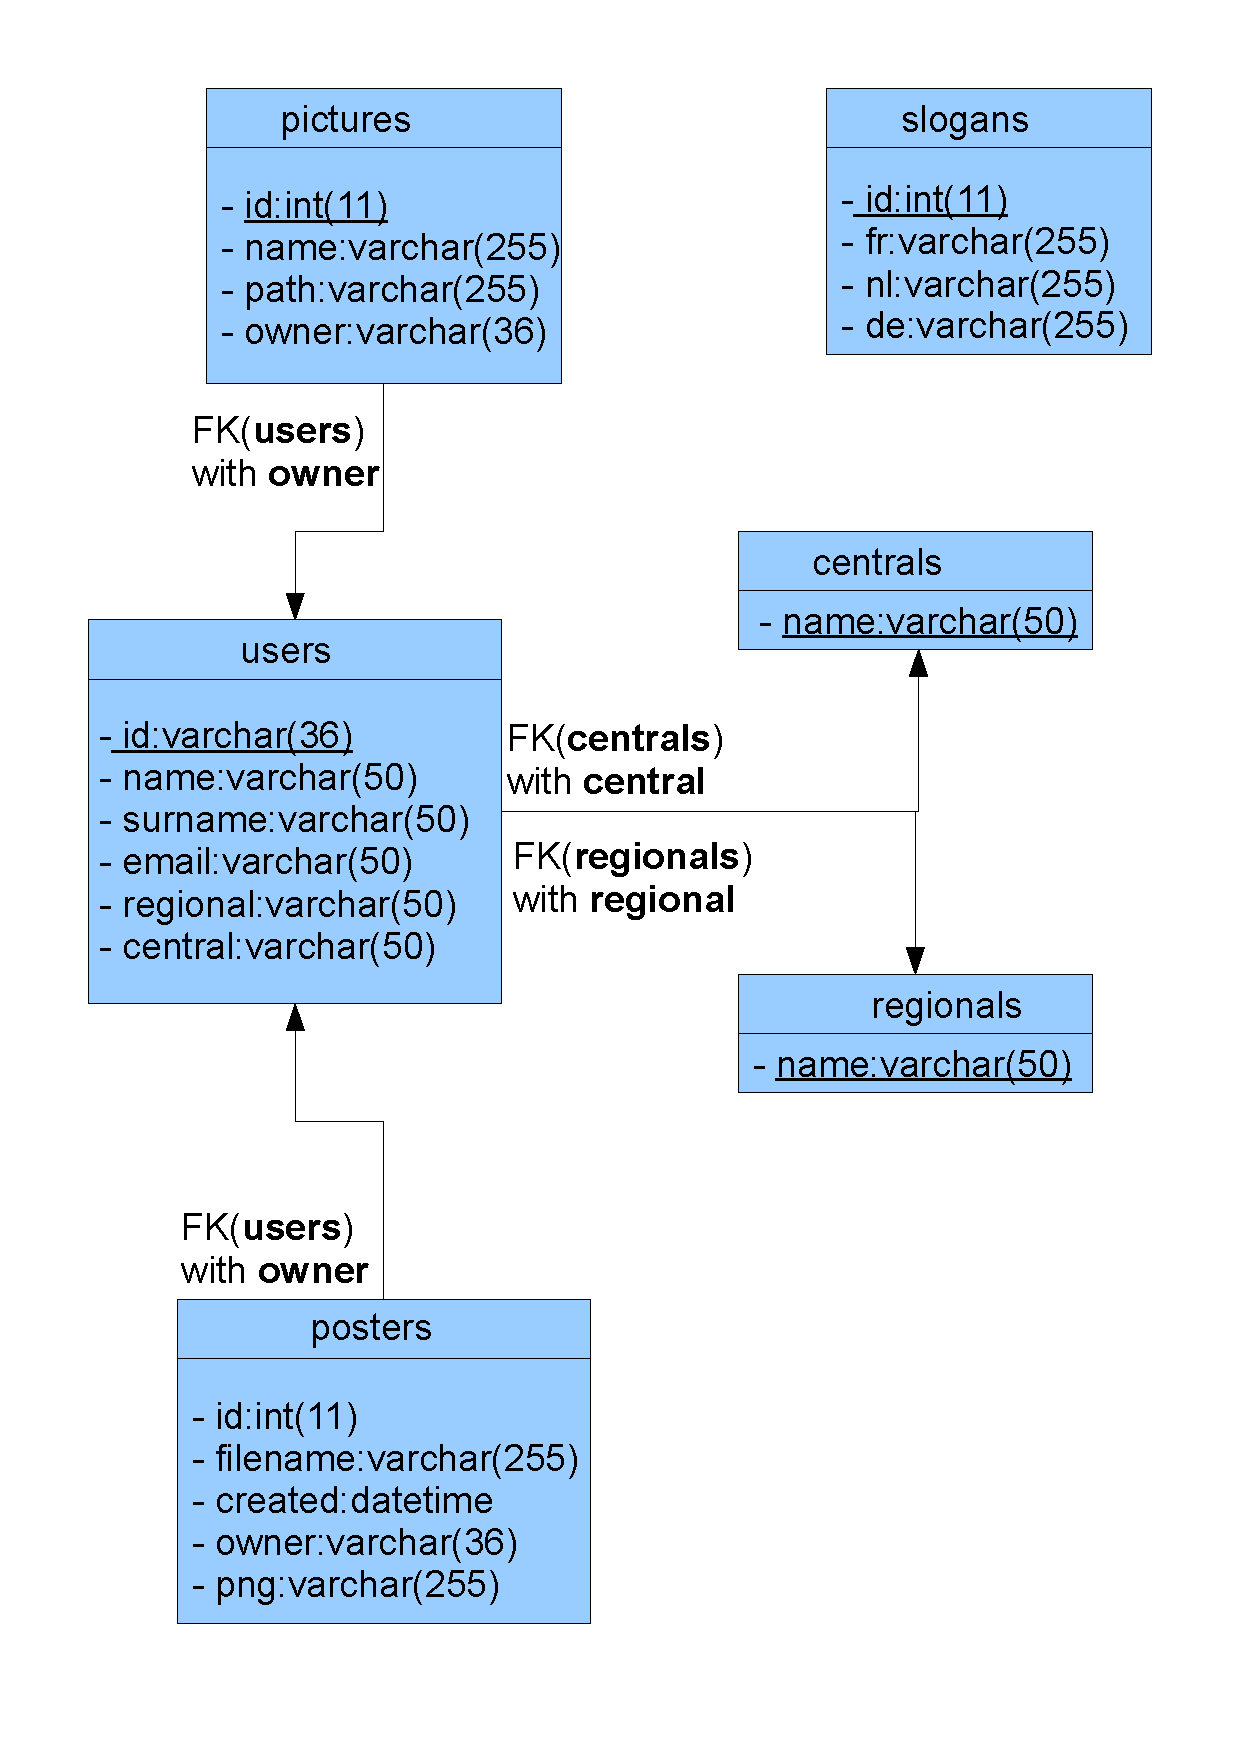
\includegraphics[width=\textwidth]{bdd.pdf} \end{center}

\newpage

\section{Annexe B : Exemples d'affiches générées par l'application}\label{exemple}

\begin{figure}[h!]
\begin{center} 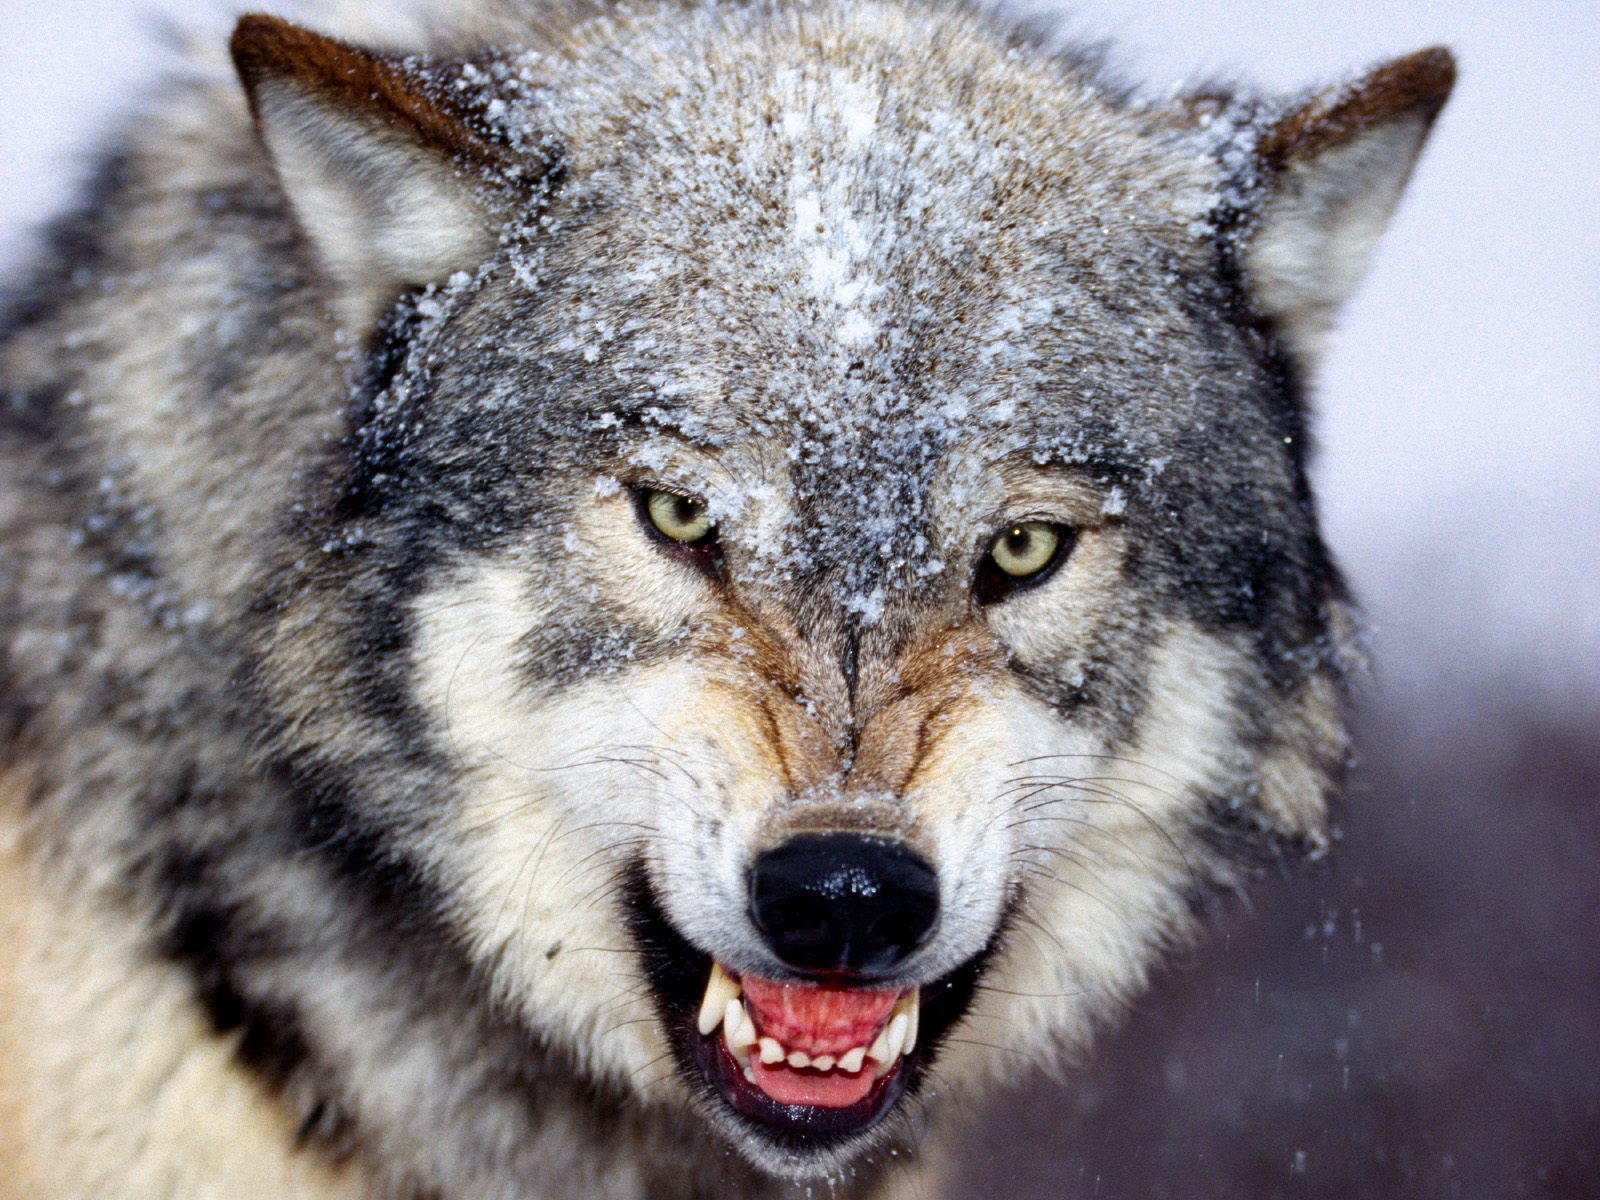
\includegraphics[height=200px]{before.jpg} \end{center}
\caption{Image initiale}
\end{figure}

\begin{figure}[h!]
\begin{center} 
\includegraphics[height=200px]{after_land.pdf} $\qquad$ 
\includegraphics[height=200px]{after_port.pdf} \end{center}
\caption{Exemples d'affiches générées}
\end{figure}

\newpage

\section{Annexe C : Timeline}\label{timeline}

\begin{figure}[!h]
	\begin{center}
		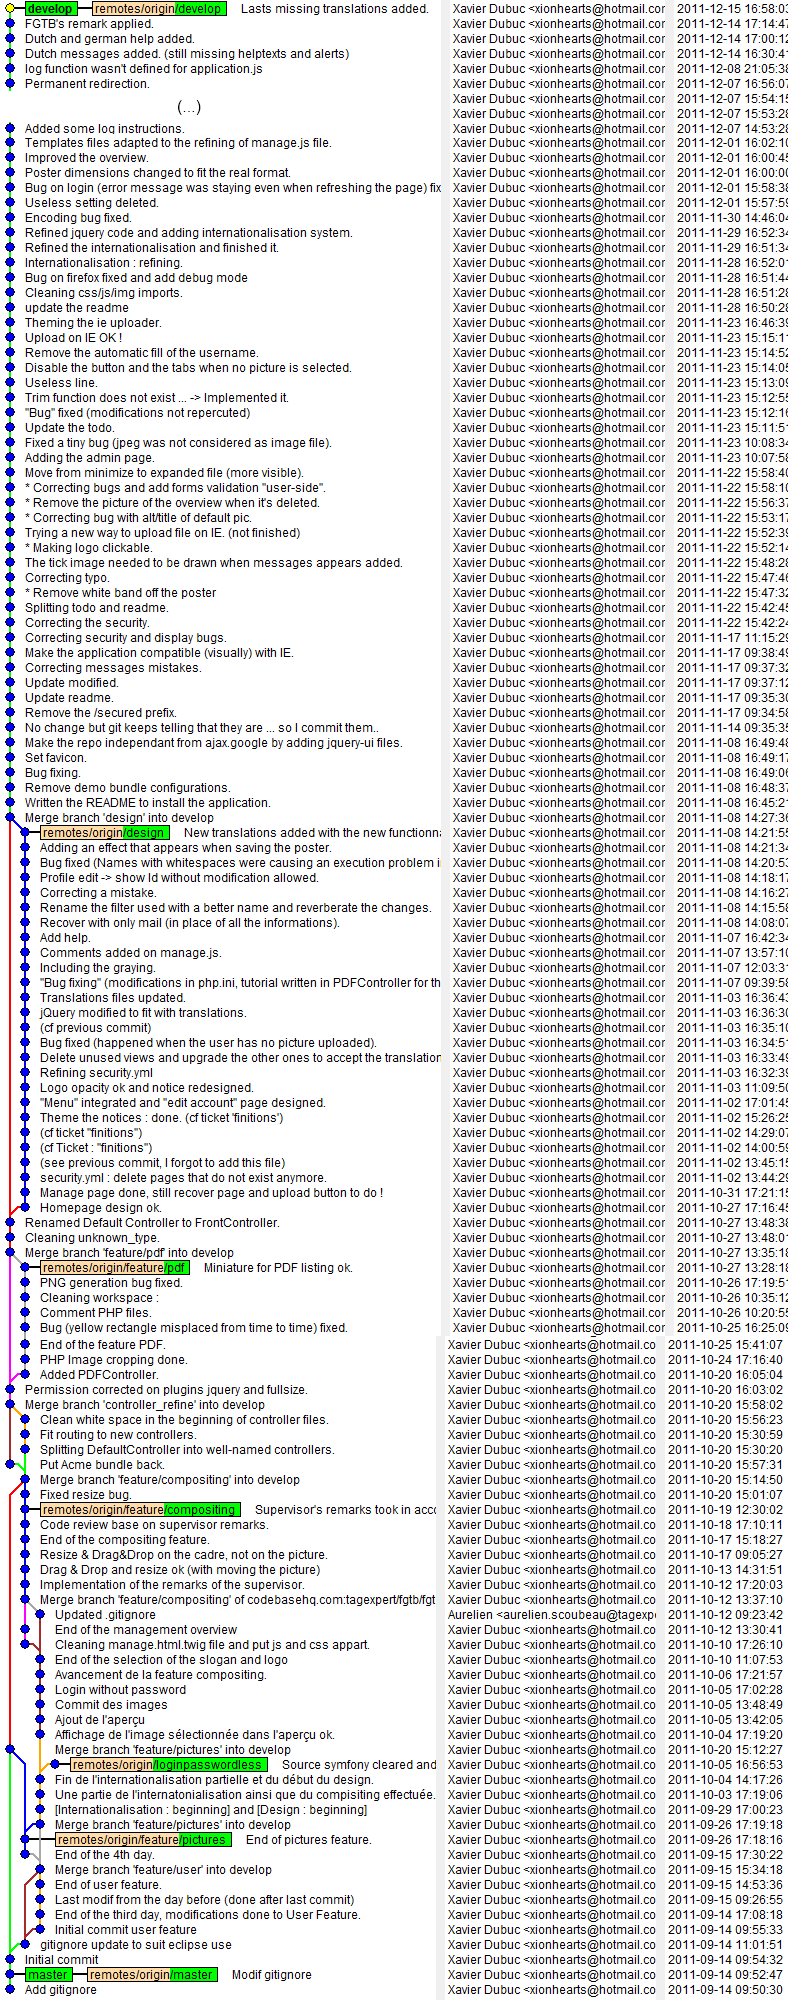
\includegraphics[height=600px]{timeline.png}
	\end{center}
	\caption{Timeline du projet}
\end{figure}

\newpage

\section{Annexe D : Descriptif des messages utilisés en screenshots}\label{messyml}

\begin{figure}[!h]
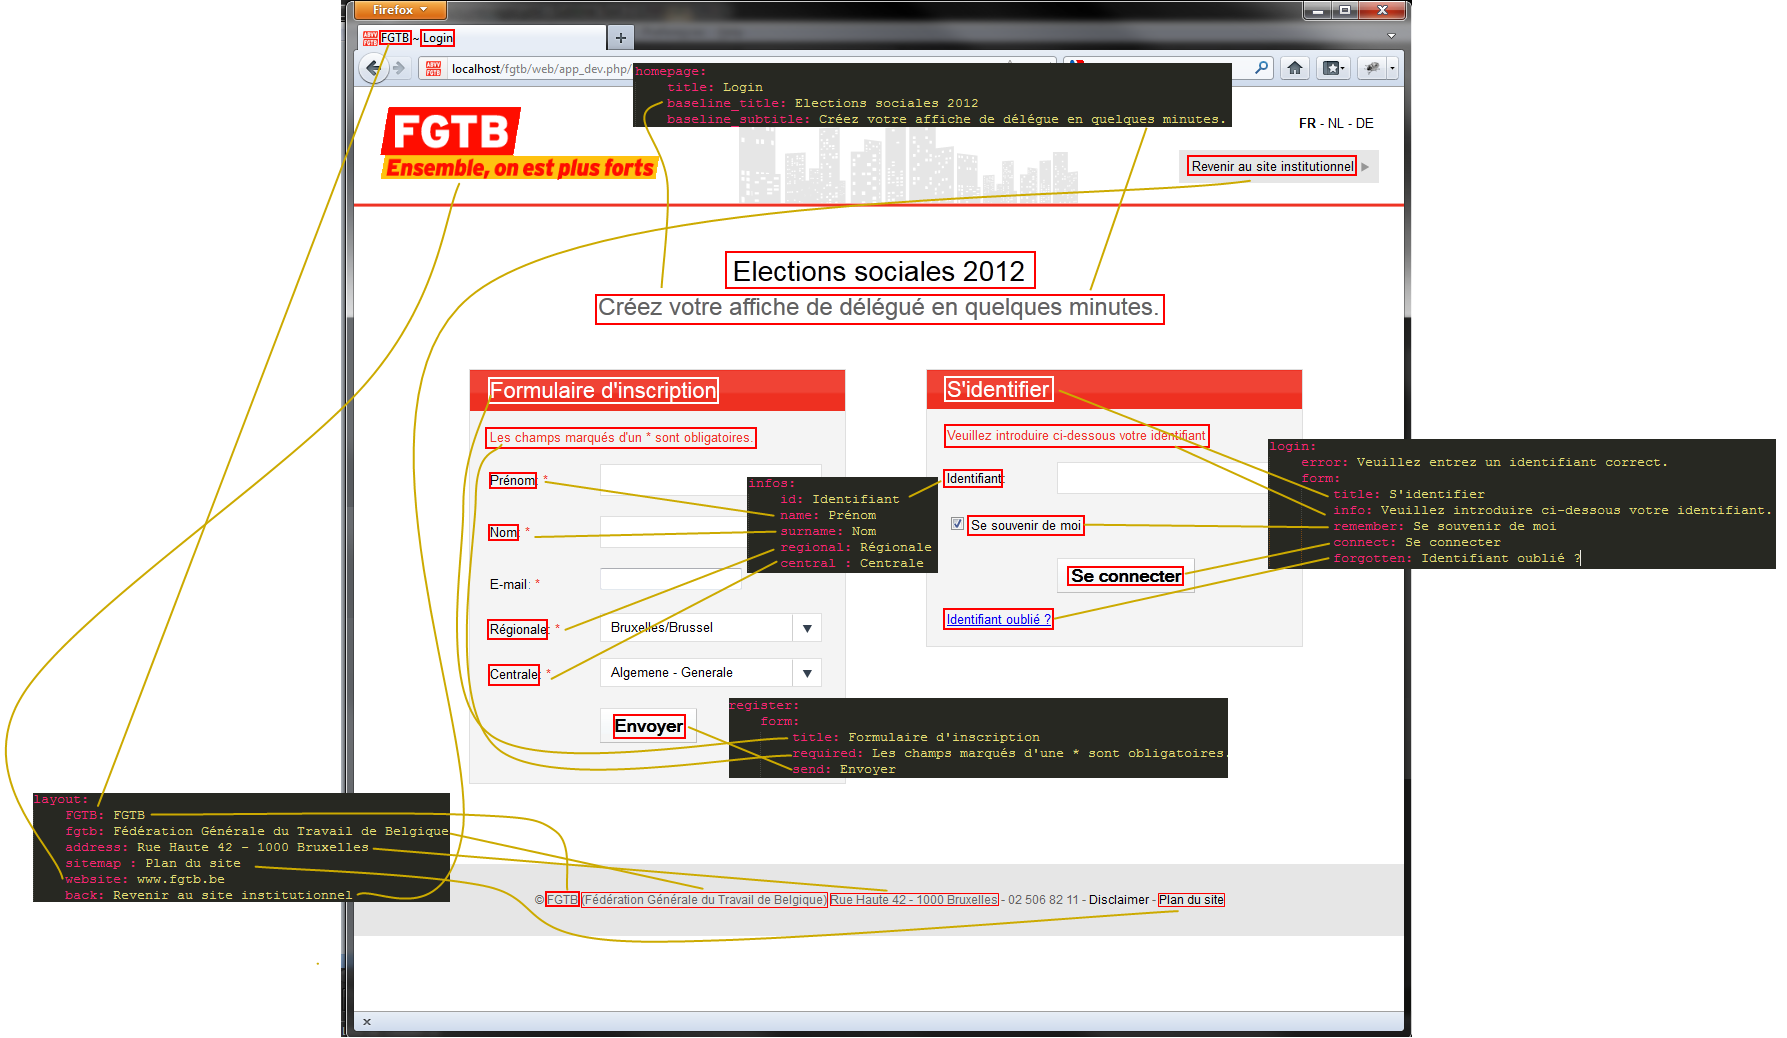
\includegraphics[width=\textwidth]{messages_homepage.png}
\caption{Page d'accueil}
\end{figure}

\begin{figure}[!h]
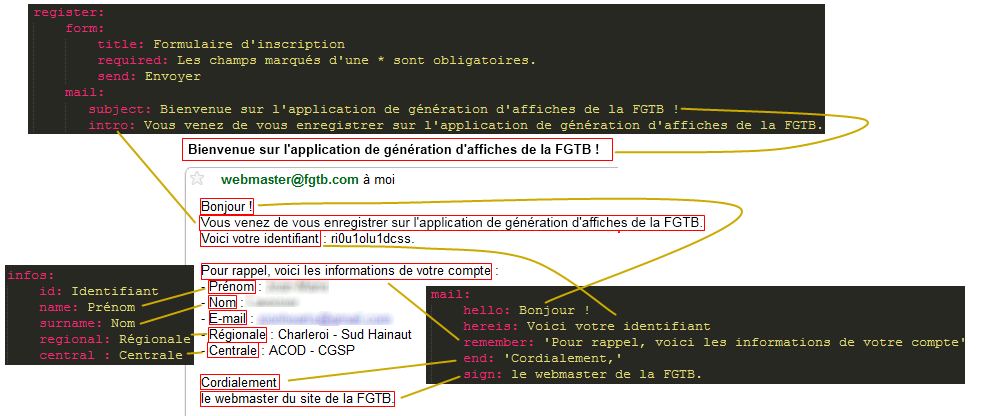
\includegraphics[width=\textwidth]{messages_registermail.png}
\caption{Mail d'inscription}
\end{figure}

\begin{figure}[!h]
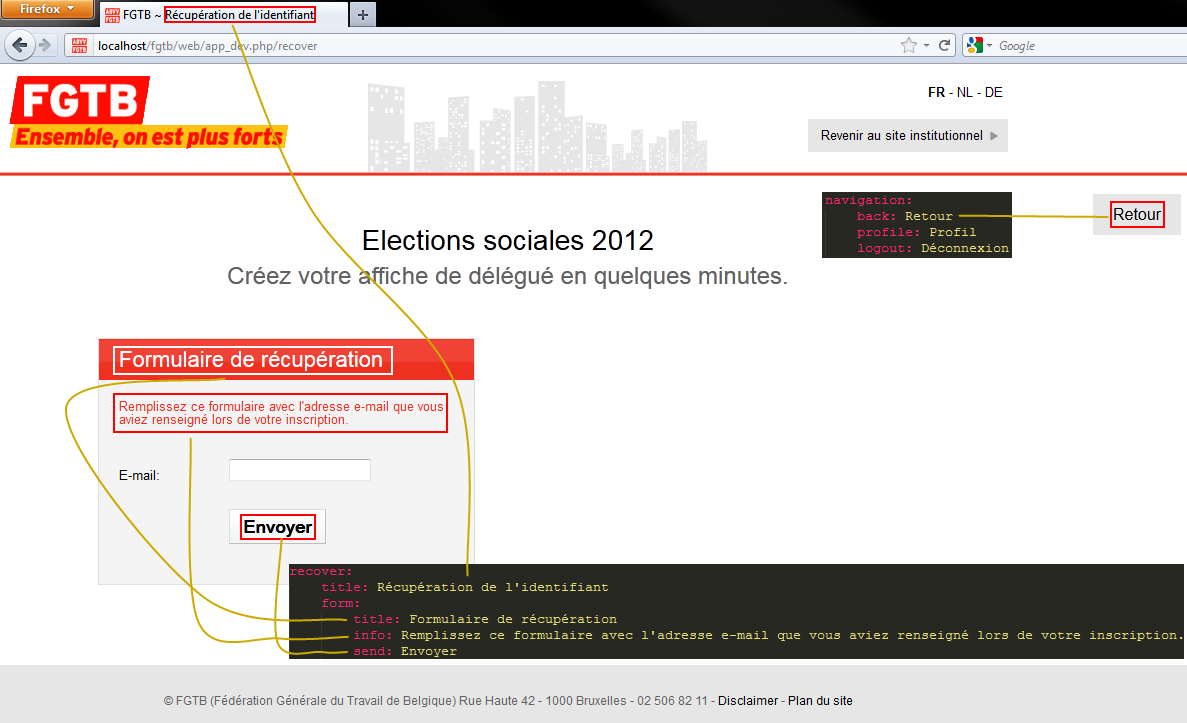
\includegraphics[width=\textwidth]{messages_recoverpage.png}
\caption{Page de récupération de l'identifiant}
\end{figure}

\begin{figure}[!h]
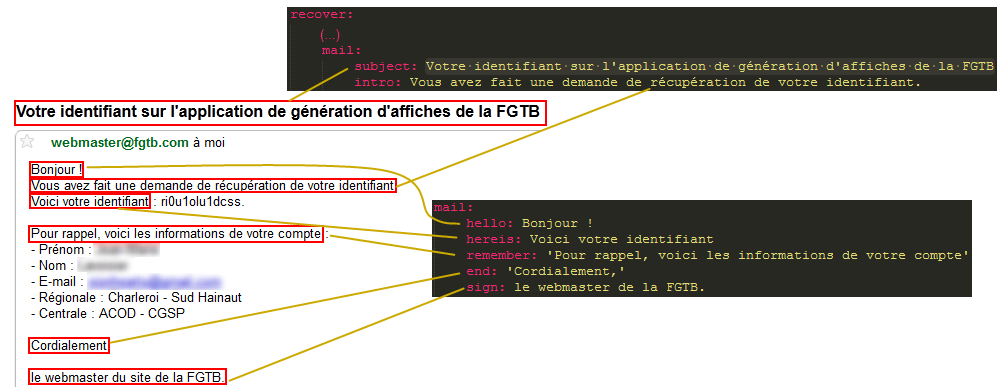
\includegraphics[width=\textwidth]{messages_recovermail.png}
\caption{Mail de récupération de l'identifiant}
\end{figure}

\begin{figure}[!h]
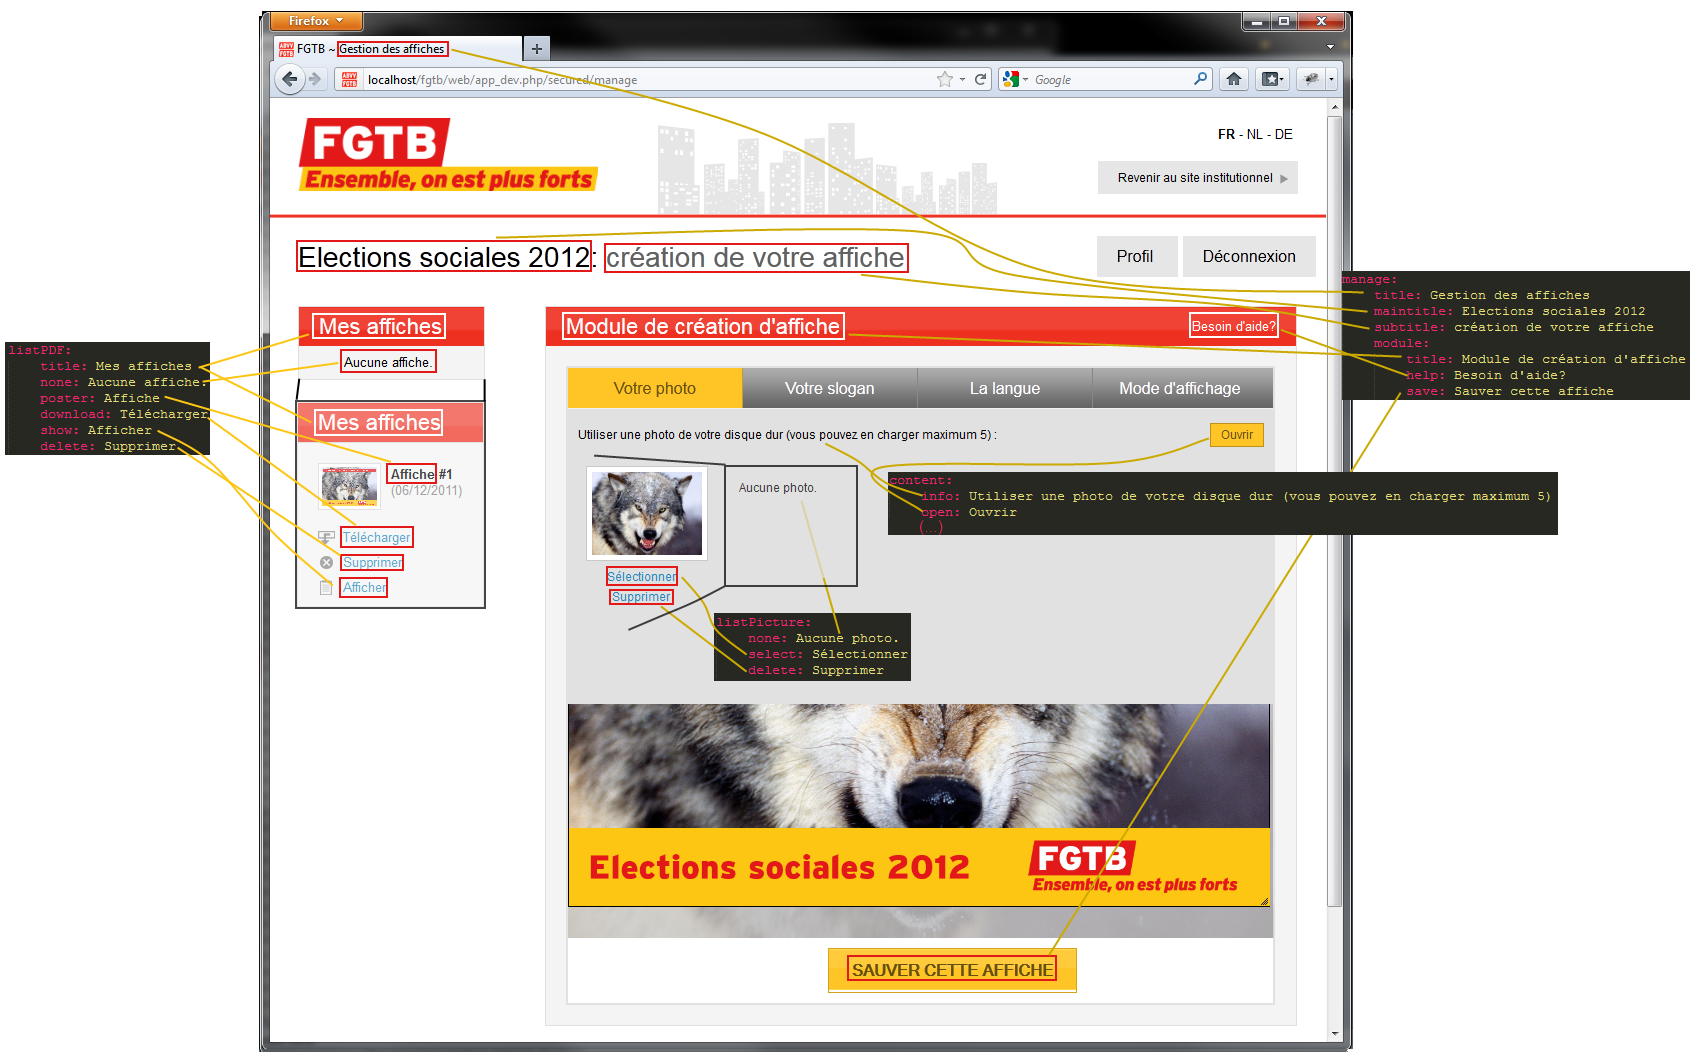
\includegraphics[angle=-90,width=\textwidth]{messages_manage_step1.png}
\caption{Page de gestion des affiches : partie 1}
\end{figure}

\begin{figure}[!h]
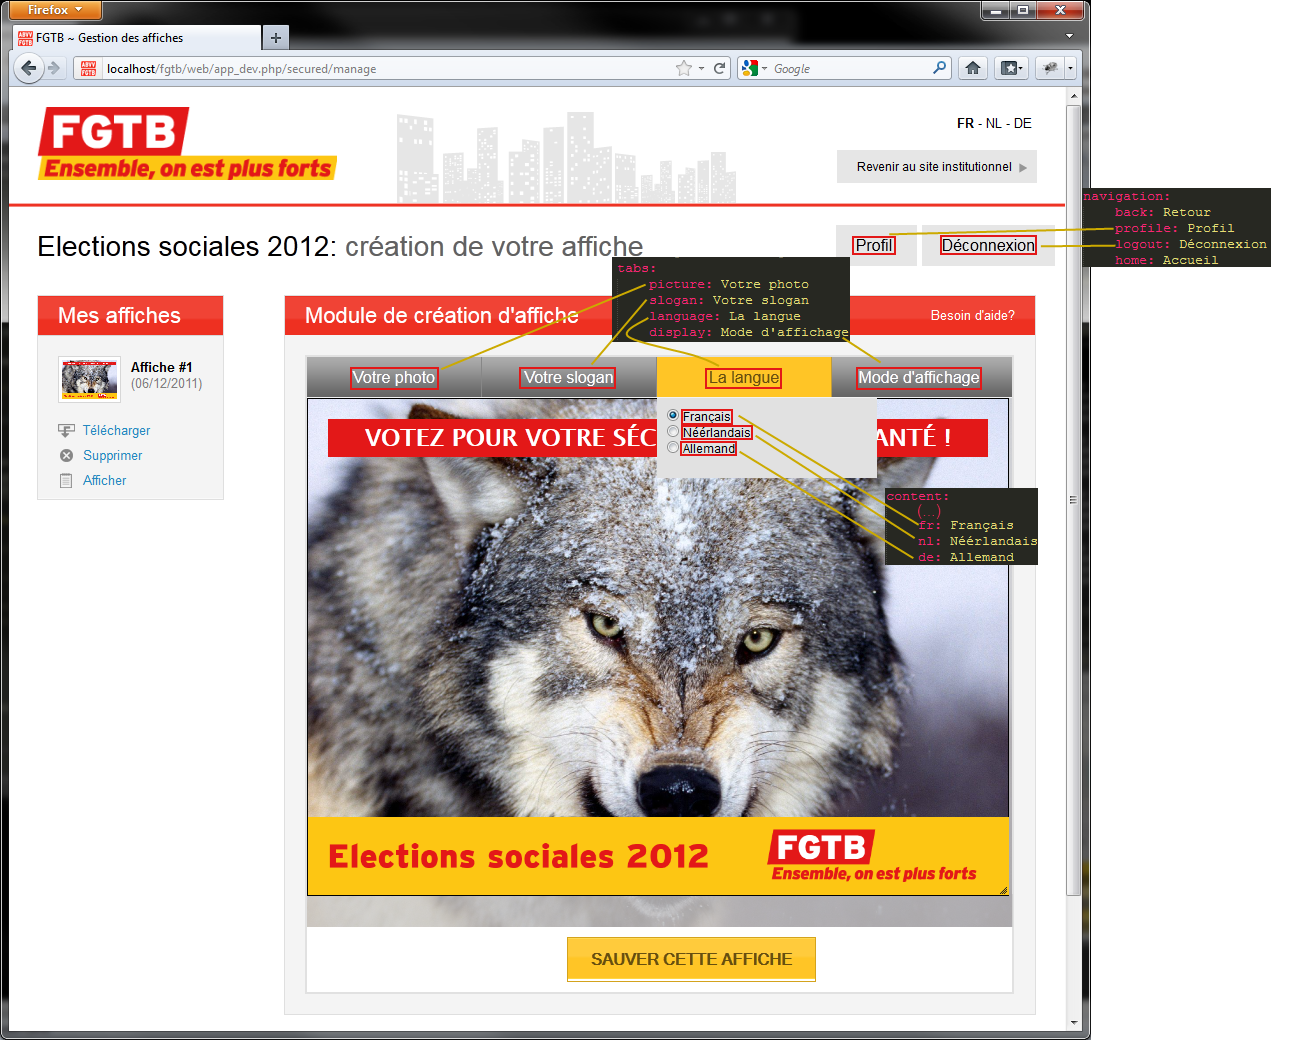
\includegraphics[angle=-90,width=\textwidth]{messages_manage_step2.png}
\caption{Page de gestion des affiches : partie 2}
\end{figure}

\begin{figure}[!h]
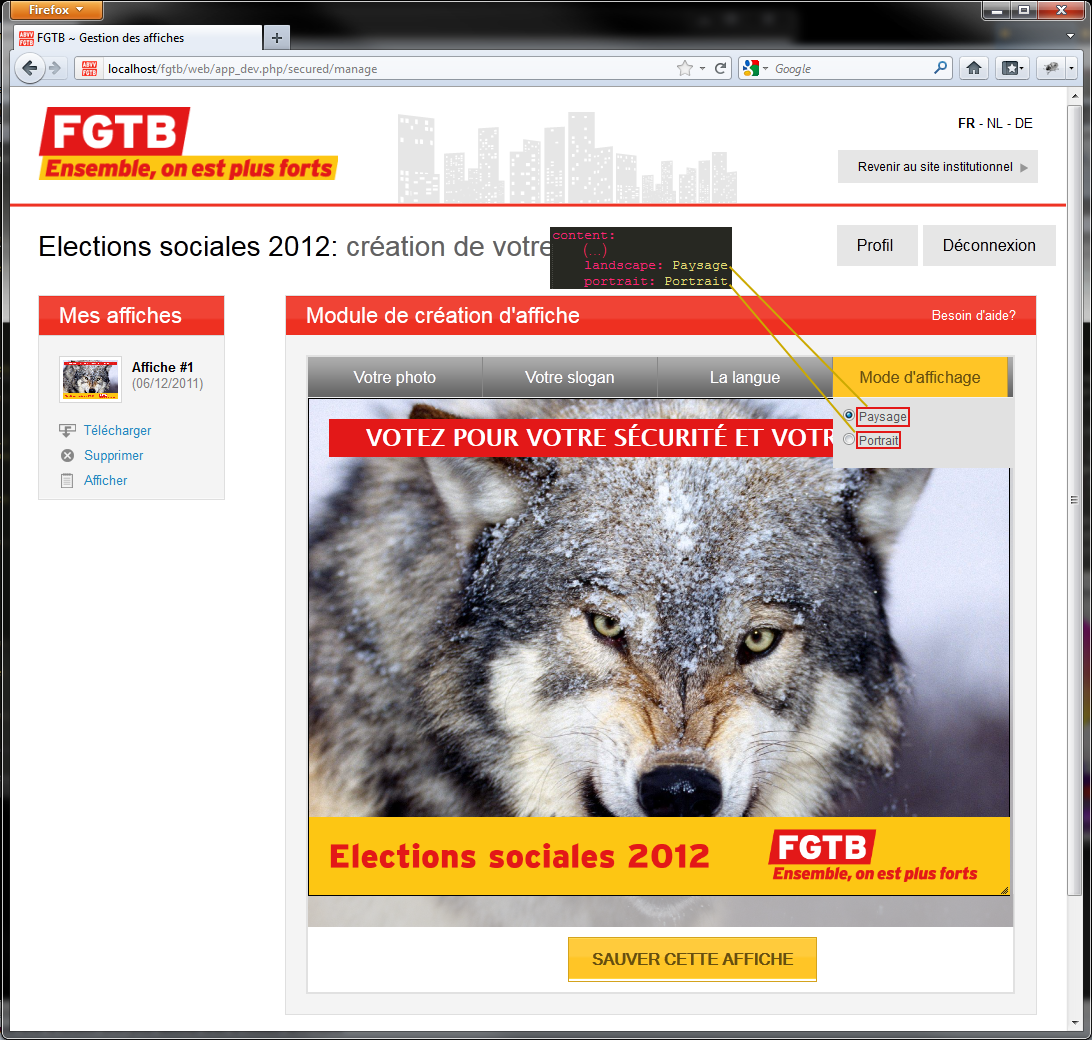
\includegraphics[angle=-90,width=\textwidth]{messages_manage_step3.png}
\caption{Page de gestion des affiches : partie 3}
\end{figure}

\begin{figure}[!h]
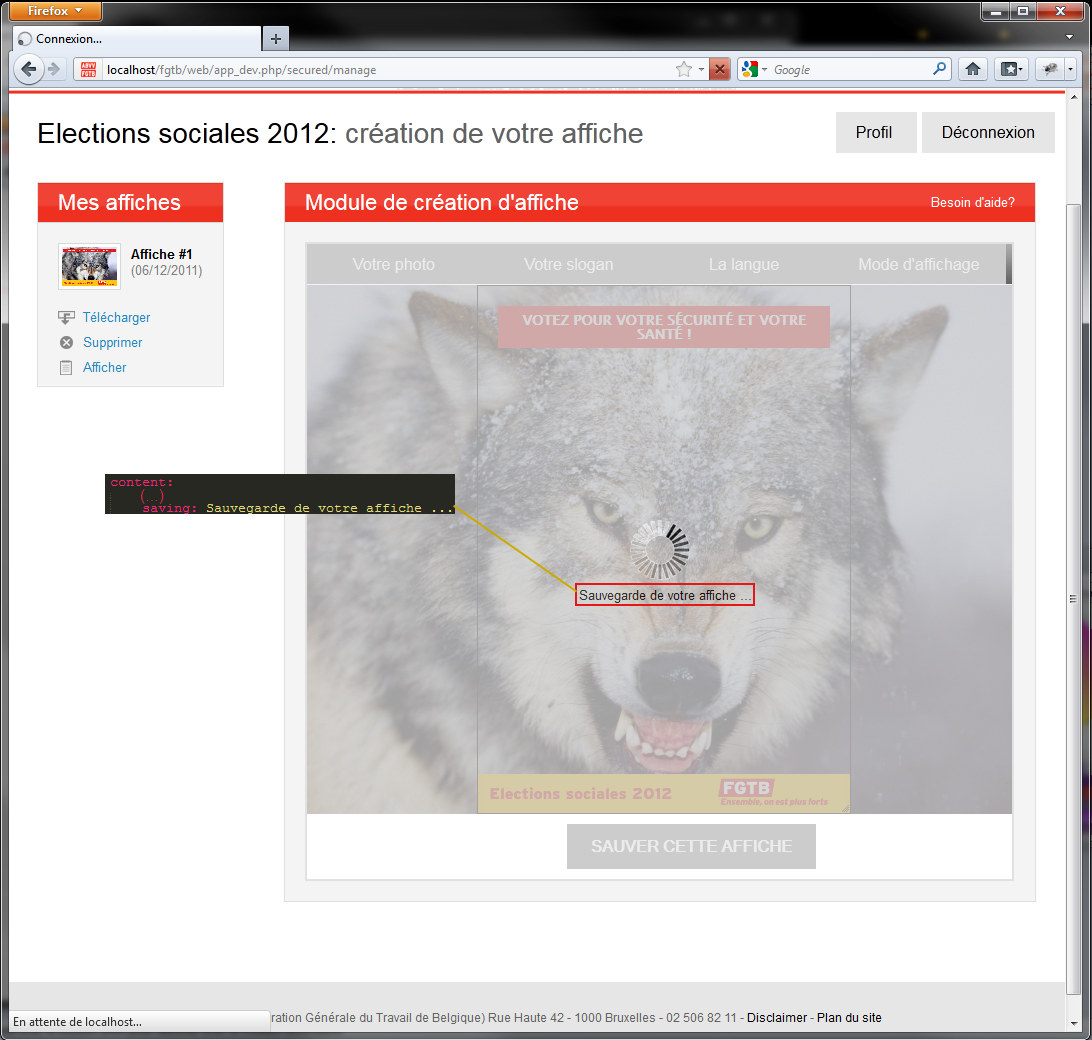
\includegraphics[angle=-90,width=\textwidth]{messages_manage_step4.png}
\caption{Page de gestion des affiches : partie 4}
\end{figure}

\begin{figure}[!h]
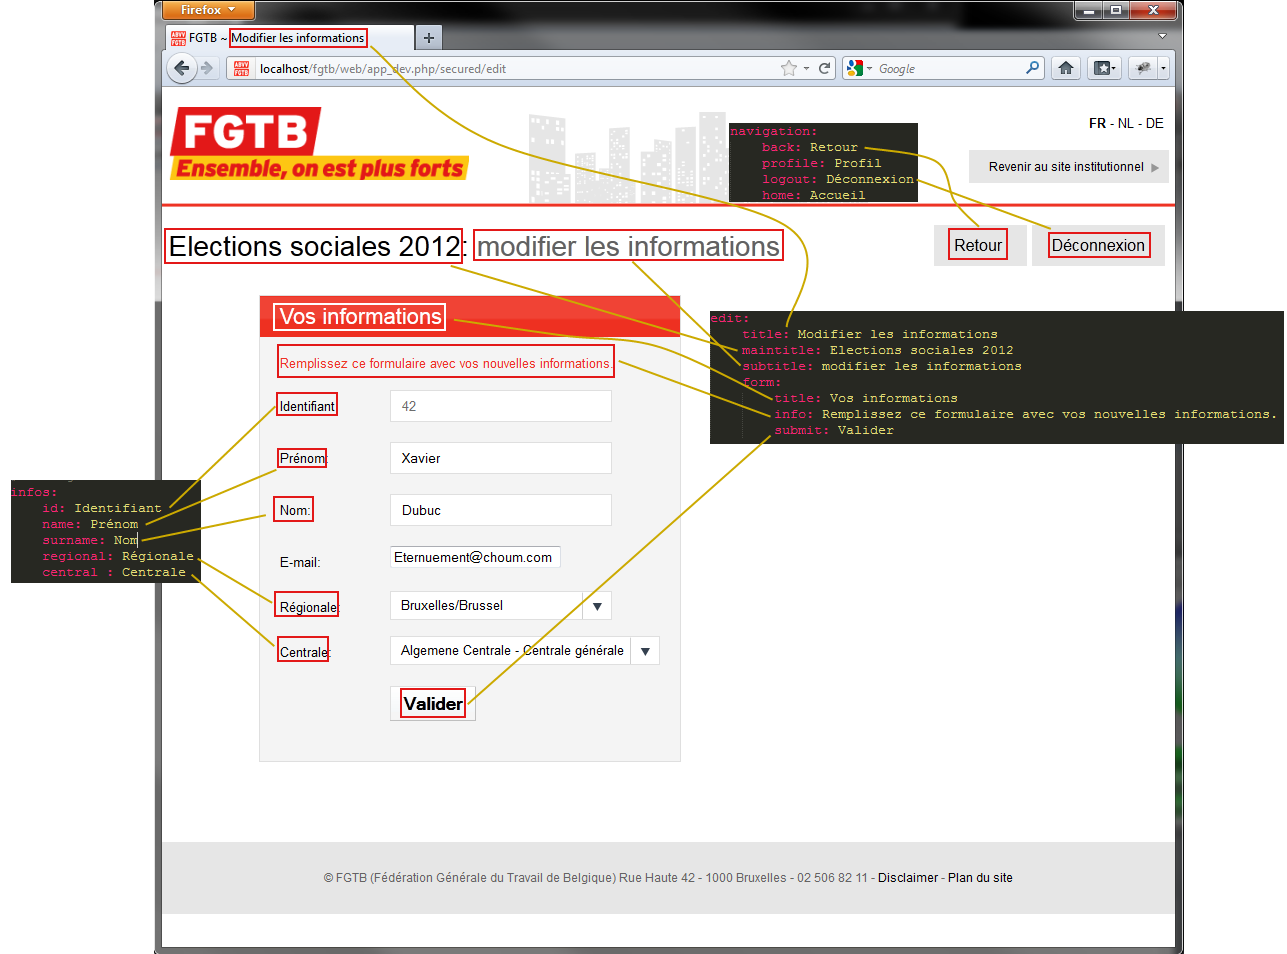
\includegraphics[angle=-90,width=\textwidth]{messages_profile.png}
\caption{Page d'édition du profil}
\end{figure}

\begin{figure}[!h]
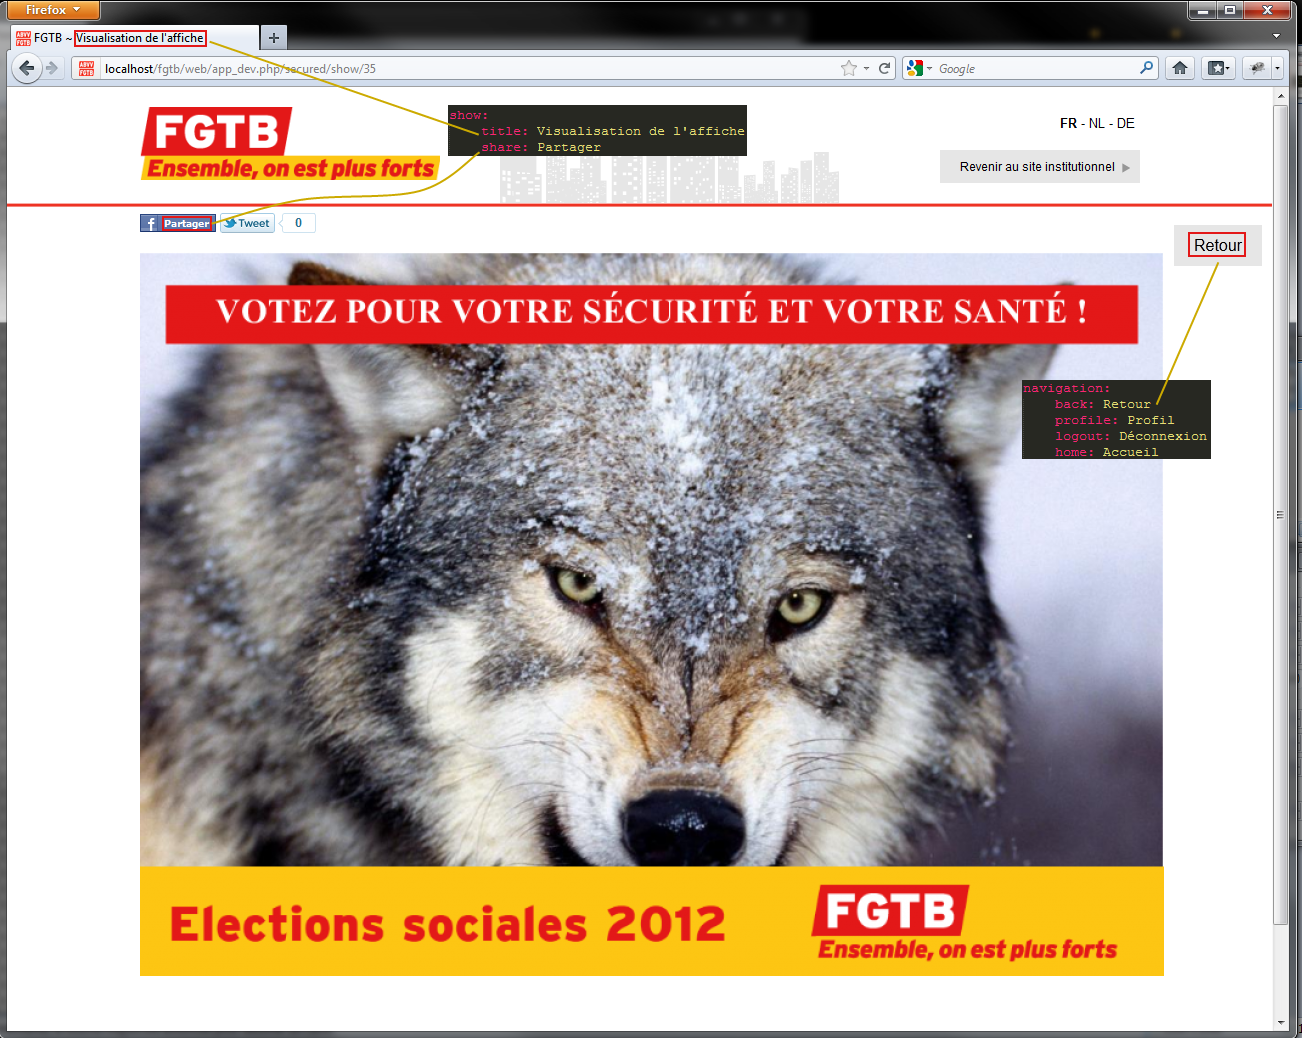
\includegraphics[angle=-90,width=\textwidth]{messages_show.png}
\caption{Page d'affichage d'une affiche en png}
\end{figure}

\begin{figure}[!h]
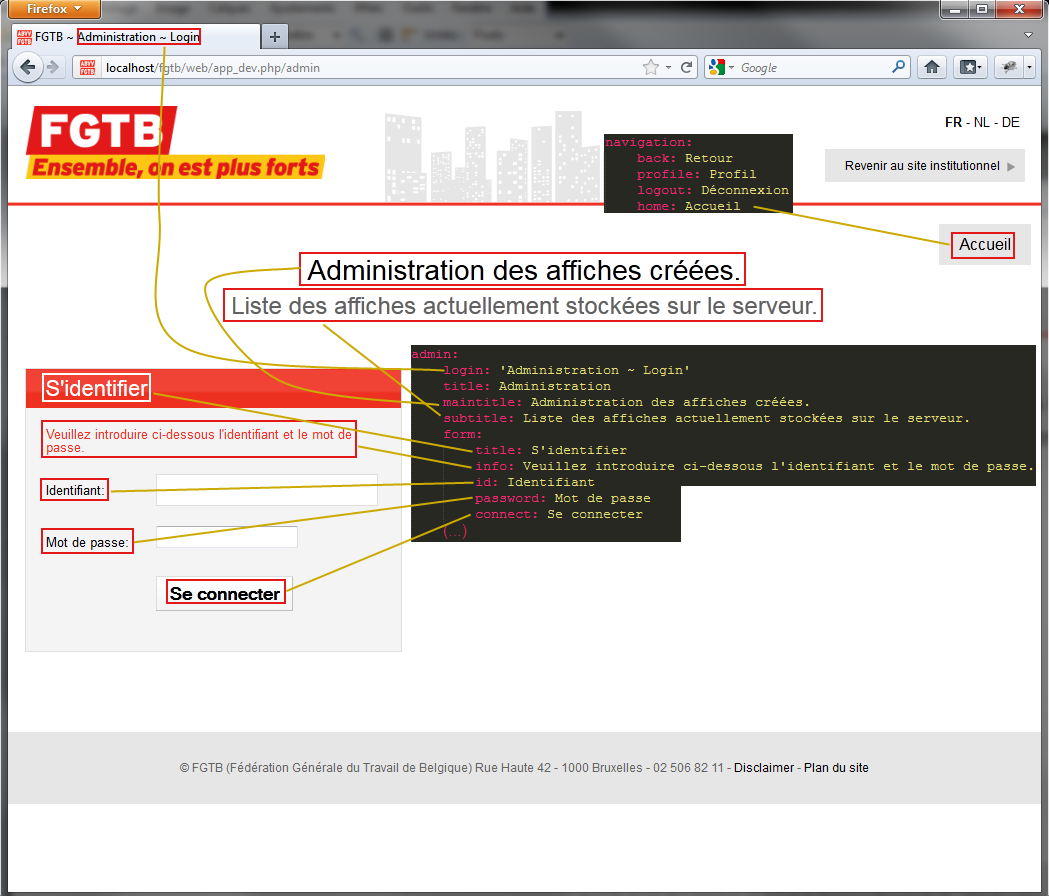
\includegraphics[angle=-90,width=\textwidth]{messages_adminlogin.png}
\caption{Page d'accueil de la partie administration}
\end{figure}

\begin{figure}[!h]
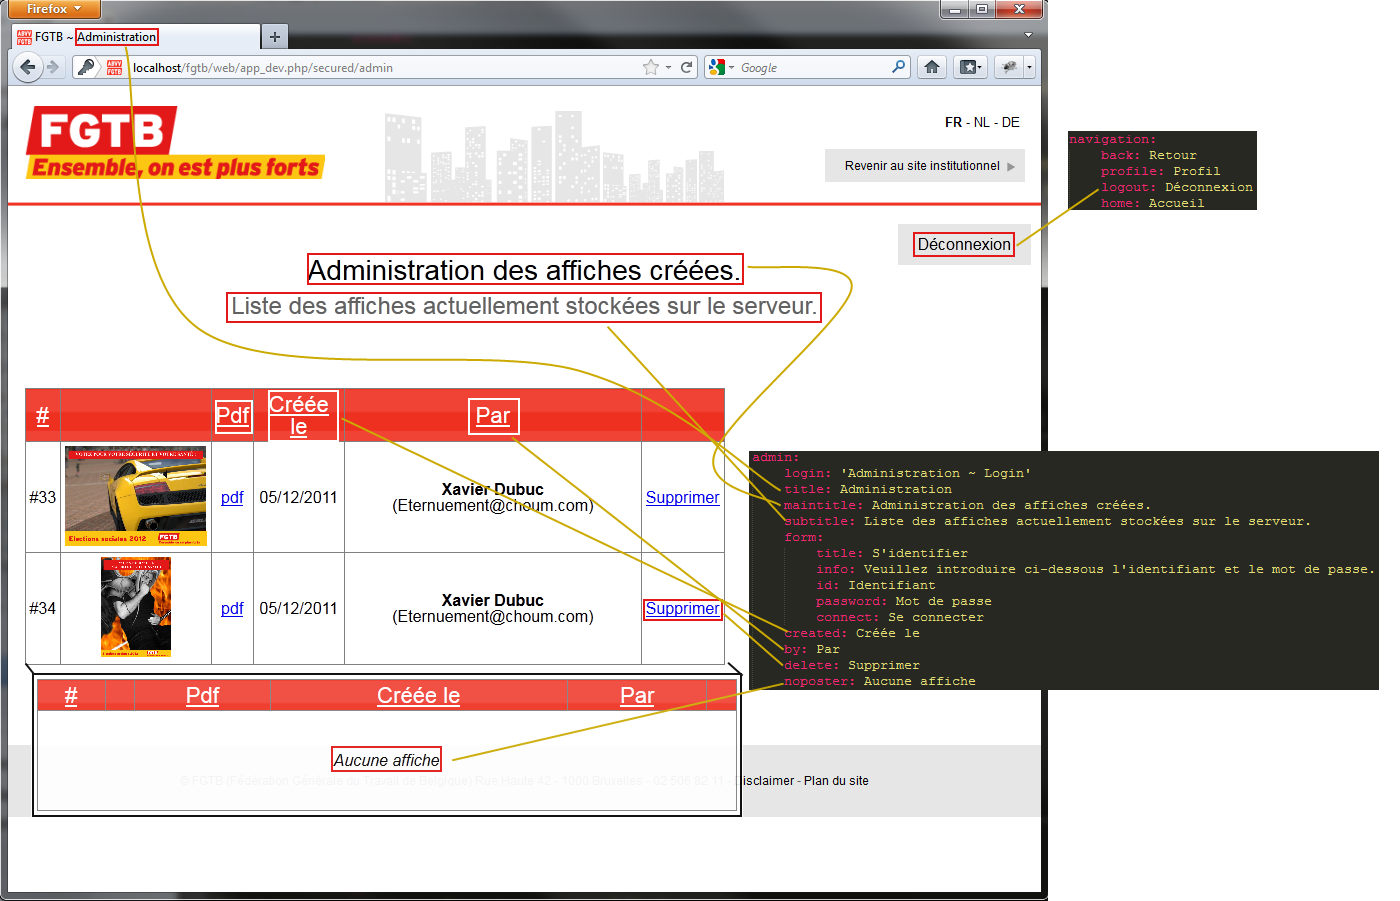
\includegraphics[angle=-90,width=\textwidth]{messages_admin.png}
\caption{Page d'administration}
\end{figure}

\end{sffamily}\end{document}